% Fakesection 序言之前
\RequirePackage[l2tabu, orthodox]{nag}
\RequirePackage{ifxetex}
\RequireXeTeX
\documentclass{ctexrep}
%颜色
\usepackage{xcolor}
%长度
\usepackage{printlen}
\uselengthunit{mm}
%图形
\usepackage{pifont}
\usepackage{ean13isbn}
\usepackage{qrcode}
\usepackage{pdfpages}
\usepackage{overpic}
\usepackage{graphicx}
\graphicspath{{./src/}}
\usepackage{media9}
\usepackage{wallpaper}
\usepackage{wrapfig}
%表格
\usepackage{tabu}
\usepackage{longtable}
\usepackage{booktabs}
\usepackage{diagbox}
\usepackage{multicol}
\usepackage{multirow}
\usepackage{makecell}
\usepackage{fancybox}
\usepackage{colortbl}
\usepackage{tcolorbox}
\tcbuselibrary{skins}
\tcbuselibrary{breakable}
\tcbuselibrary{theorems}
\tcbuselibrary{listings}
\tcbuselibrary{xparse}
\tcbuselibrary{minted}% 用minted排版代码
\usepackage{fvextra}
\usepackage{csvsimple}
\usepackage{boxedminipage2e}
%公式
\usepackage{amsmath}
\usepackage{amsthm}
\usepackage{amsfonts}
\usepackage{amssymb}
\usepackage{amsbsy}
\usepackage{amsopn}
\usepackage{amstext}
\usepackage{mathrsfs}
\usepackage{bm}
\usepackage{textcomp}
\usepackage{latexsym}
\usepackage{exscale}
\usepackage{relsize}
%\usepackage{xymtex}
\usepackage{physics}
\usepackage{siunitx}
\usepackage{hologo}
\usepackage{cases}
%文字
\usepackage{csquotes}
\usepackage{microtype}
%正文
\usepackage{fancyhdr}
\usepackage{geometry}
\usepackage{lastpage}
\usepackage{indentfirst}
\usepackage{setspace}
\renewcommand\arraystretch{1.5}
%非正文
\usepackage{makeidx}
\makeindex
\usepackage{epigraph}
\usepackage{varwidth}
\usepackage{exercise}
\usepackage{tasks}
%参考文献
\usepackage{morewrites}
\renewcommand{\thefootnote}{\fnsymbol{footnote}}
\usepackage[resetlabels]{multibib}
%标题
\usepackage{caption}
\usepackage{subcaption}
\DeclareCaptionLabelFormat{andtable}%
{#1#2~\&~\tablename\thetable}
\newcounter{sub}
%其它
\usepackage{atbegshi}
\usepackage{lipsum}
\csname
endofdump
\endcsname
%非正文
\renewcommand{\ExerciseName}{问题}
\renewcommand{\AnswerName}{回答}
\renewcommand{\listexercisename}{\Huge 问题}
\numberwithin{Exercise}{chapter}
\numberwithin{Answer}{chapter}
%代码
\usepackage{minted}
\usepackage{boxie}
\makeatletter
\xdefinecolor{tcbcol@back}{rgb}{0,0,0}
\makeatother
\usepackage{tikz}
%%MatLab命令行
\newcommand{\MatlabLogo}{%
	\begin{tikzpicture}[x=2.4ex,y=2.4ex,line width=0ex,scale=1]
		\node[draw,fill=white,text=white] at (0, 0) (a) {
				\includegraphics[width=2.4ex]{matlabLogo.ai}
			};
	\end{tikzpicture}
}
\tcbset{%
	skin=enhanced,%
	matlab/.style={%
		skin=bicolor,%
		boxrule=0.1mm,%
		%toptitle=1ex,
		sharp corners,
		breakable,%
		colbacktitle=WinGray,%
		colframe=WinGray,%
		coltitle=black,%
		fonttitle=\sffamily,%\bfseries,
		fontupper=\small\sffamily,
		fontlower=\small\sffamily,
		frame style={%
			draw=WinBlue,%
			left color=WinBlue,%
			right color=WinBlue%
		},%
		overlay unbroken = {%
			\node[inner sep=0pt,anchor=north west,yshift=-3pt,xshift=1.2pt,text=black]
			at (frame.north west){\MatlabLogo};% \fbox{\faTerminal}
			\node[inner sep=0pt,anchor=north east,yshift=-3pt,xshift=-8pt,text=black] at (frame.north
			east){\rule{0.8em}{0.6pt}\quad$\square$\quad{\Large$\times$}};
		},%
		overlay first = {%
			\node[inner sep=0pt,anchor=north west,yshift=-3pt,xshift=1.0pt,text=black]
			at (frame.north west){\MatlabLogo};%\small ~\faWindows
			\node[inner sep=0pt,anchor=north east,yshift=-3pt,xshift=-8pt,text=black] at (frame.north
			east){\rule{0.8em}{0.6pt}\quad$\square$\quad{\Large$\times$}};
		}%
	},
	matlablight/.style={
		matlab,%
		colback=white,%
		colupper=black,%
		%coltext=black%
	},
	matlabdark/.style={
		matlab,%
		colback=black,%
		colupper=white,%
		%coltext=white%
	}
}
\DeclareTCBListing{matlabdarkc}{ m m }{%
	listing engine=minted,%
	minted style=trac,%
	minted options={%
		autogobble,%
		breaklines,%
		fontsize=\wuhao,%
		baselinestretch=0.6,%
		breaksymbolleft={},%
		numbersep=3mm%
	},%
	listing and comment,%
	colbacklower=tcbcol@back!5!yellow!10!white,%
	collower=linux,%
	matlabdark,%
	title={#2},%
	comment={\small\sffamily#1},%
	minted language=bat%
}
\DeclareTCBListing{matlablightc}{ m m }{%
	listing engine=minted,%
	minted style=trac,%
	minted options={%
		autogobble,%
		breaklines,%
		fontsize=\wuhao,%
		baselinestretch=0.6,%
		breaksymbolleft={},%
		numbersep=3mm%
	},%
	listing and comment,%
	colbacklower=tcbcol@back!5!yellow!10!white,%
	collower=linux,%
	matlablight,%
	title={#2},%
	comment={\small\sffamily#1},%
	minted language=bat%
}
\DeclareTCBListing{matlabdark}{ m }{%
	listing engine=minted,%
	minted style=trac,%
	minted options={%
		autogobble,%
		breaklines,%
		fontsize=\wuhao,%
		baselinestretch=0.6,%
		breaksymbolleft={},%
		numbersep=3mm%
	},%
	listing only,%
	matlabdark,%
	title={#1},%
	minted language=bat%
}
\DeclareTCBListing{matlablight}{ m }{%
	listing engine=minted,%
	minted style=trac,%
	minted options={%
		autogobble,%
		breaklines,%
		fontsize=\wuhao,%
		baselinestretch=0.6,%
		breaksymbolleft={},%
		numbersep=3mm%
	},%
	listing only,%
	matlablight,%
	title={#1},%
	minted language=bat%
}
\newtcbinputlisting{\matlabdarkcfile}[3]{%
	listing engine=minted,%
	minted style=trac,%
	minted options={%
		autogobble,%
		breaklines,%
		fontsize=\wuhao,%
		baselinestretch=0.6,%
		breaksymbolleft={},%
		numbersep=3mm%
	},%
	listing and comment,%
	colbacklower=tcbcol@back!5!yellow!10!white,%
	collower=linux,%
	matlabdark,%
	listing file={#3},
	title={#2},%
	comment={\small\sffamily#1},%
	minted language=bat%
}% end matlabdarkcfile
% 将文件做为窗口内容的Windows终端窗口样式命令
% 第1个参数是窗口底端提示信息
% 第2个参数是窗口标题
% 第3个参数是包含窗口内容的文件全路径名称(可以是相对路径)
\newtcbinputlisting{\matlablightcfile}[3]{%
	listing engine=minted,%
	minted style=trac,%
	minted options={%
		autogobble,%
		breaklines,%
		fontsize=\wuhao,%
		baselinestretch=0.6,%
		breaksymbolleft={},%
		numbersep=3mm%
	},%
	listing and comment,%
	colbacklower=tcbcol@back!5!yellow!10!white,%
	collower=linux,%
	matlablight,%
	listing file={#3},
	title={#2},%
	comment={\small\sffamily#1},%
	minted language=bat%
}% end matlablightcfile
% 将文件做为窗口内容的Windows终端窗口样式命令
% 第1个参数是窗口标题
% 第2个参数是包含窗口内容的文件全路径名称(可以是相对路径)
\newtcbinputlisting{\matlabdarkfile}[2]{%
	listing engine=minted,%
	minted style=trac,%
	minted options={%
		autogobble,%
		breaklines,%
		fontsize=\wuhao,%
		baselinestretch=0.6,%
		breaksymbolleft={},%
		numbersep=3mm%
	},%
	listing only,%
	matlabdark,%
	listing file={#2},
	title={#1},%
	minted language=bat%
}% end matlabdarkfile
% 将文件做为窗口内容的Windows终端窗口样式命令
% 第1个参数是窗口标题
% 第2个参数是包含窗口内容的文件全路径名称(可以是相对路径)
\newtcbinputlisting{\matlablightfile}[2]{%
	listing engine=minted,%
	minted style=trac,%
	minted options={%
		autogobble,%
		breaklines,%
		fontsize=\wuhao,%
		baselinestretch=0.6,%
		breaksymbolleft={},%
		numbersep=3mm%
	},%
	listing only,%
	matlablight,%
	listing file={#2},
	title={#1},%
	minted language=bat%
}% end matlablightfile
%链接%与beamer 冲突
\usepackage
[	colorlinks = true,
linkcolor = gray,
citecolor = gray,
backref=page
]{hyperref}
%枚举%与beamer 干涉
\usepackage{enumitem}
\setlist[enumerate, 2]
{	fullwidth,
	label = \alph*.,
	font = \textup,
	itemindent=2em
}
%标题%与beamer 冲突
\usepackage{titlesec}
\titleformat{\chapter}{\centering\Huge\bfseries}{实验\chinese{chapter}~}{0pt}{}
%\titleformat{\section}{\centering\LARGE\bfseries}{\S\ifthenelse{\value{section}=0}{}{\thesection}~}{0pt}{}
%\titleformat{\subsection}{\Large}{\chinese{subsection}、~}{0pt}{}
%\titleformat{\subsubsection}{\large}{\arabic{subsubsection}.~}{0pt}{}
\begin{document}
% Fakesection 扉页
\begin{titlepage}
	\centering
	\includegraphics[width=.8\linewidth]{NJUST.ai}
	\vspace{20mm}
	\textbf{\heiti\zihao{1}信号与系统}
	\vspace{5mm}
	\textbf{\heiti\zihao{1}实验报告}
	\vspace{30mm}
	\begin{spacing}{1}
		\centering
		\zihao{3}
		\begin{tabu}to.8\linewidth{@{}X[4,r]@{}X[c]@{}X[12,l]@{}}
			\makebox[4\ccwd][s]{学院}&:&\underline{\makebox[12\ccwd][c]{\kaishu{电子工程与光电技术学院}}}\\
			\makebox[4\ccwd][s]{班号}&:&\underline{\makebox[12\ccwd][c]{\kaishu{9171040G11}}}\\
			\makebox[4\ccwd][s]{姓名}&:&\underline{\makebox[12\ccwd][c]{\kaishu{吴振宇}}}\\
			\makebox[4\ccwd][s]{学号}&:&\underline{\makebox[12\ccwd][c]{\kaishu{916101630117}}}\\
			\makebox[4\ccwd][s]{同组同学}&:&\underline{\makebox[12\ccwd][c]{\kaishu{毛东兴}}}\\
			\makebox[4\ccwd][s]{学号}&:&\underline{\makebox[12\ccwd][c]{\kaishu{9171160D0529}}}\\
			\makebox[4\ccwd][s]{指导老师}&:&\underline{\makebox[12\ccwd][c]{\kaishu{王海青}}}
		\end{tabu}
	\end{spacing}
	\vspace{10mm}
	\zihao{3}
	\kaishu{\today}
\end{titlepage}
%页眉页脚%与book冲突
\pagestyle{fancy}
\renewcommand{\headrulewidth}{0pt}
\lhead{}
\chead{}
\rhead{}
\lfoot{\small{\leftmark}}
\cfoot{\small{第\thepage 页~共~\pageref{LastPage}~页}}
\rfoot{\small{\rightmark}}
% Fakesection 目录
\pagenumbering{roman}
\tableofcontents
\newpage
\listoffigures
\newpage
\listoftables
\newpage
\listofexercises
\newpage
\pagenumbering{arabic}
\chapter{周期信号的频谱测试}%
\label{cha:周期信号的频谱测试}

\section{实验目的}%
\label{sec:实验目的\arabic{chapter}}

\begin{enumerate}
	\item 掌握周期信号频谱的测试方法;
	\item 了解典型信号频谱的特点,建立典型信号的波形与频谱之间的关系。
\end{enumerate}

\section{实验原理及方法}%
\label{sec:实验原理及方法\arabic{chapter}}

\begin{enumerate}
	\item 信号的频谱可分为幅度谱、相位谱和功率谱,分别是将信号的基波和各次谐波的振幅、相位和功率按频率的高低依次排列而成的图形。
	\item 连续时间信号的频谱具有离散性、谐波性、收敛性。

		例如正弦波、周期矩形脉冲、三角波的幅度谱分别如图\ref{fig:正弦波波形和幅度谱}、\ref{fig:周期矩形脉冲的波形和幅度谱}、\ref{fig:三角波的波形和幅度谱}所示:

		\begin{enumerate}
			\item 正弦波的幅度谱如图\ref{fig:正弦波波形和幅度谱}所示。

				\begin{figure}[htpb]
					\centering
					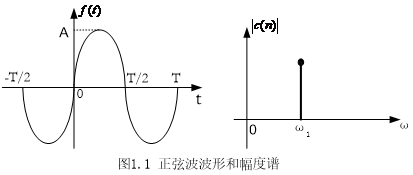
\includegraphics[width=0.8\linewidth]{1-2.png}
					\caption{正弦波波形和幅度谱}
					\label{fig:正弦波波形和幅度谱}
				\end{figure}

			\item 周期矩形脉冲的幅度谱如图\ref{fig:周期矩形脉冲的波形和幅度谱}所示。周期矩形脉冲的周期$ T $变化和$ \tau $变化时,幅度谱如图\ref{fig:周期矩形脉冲的波形和幅度谱的变化}所示。

				\begin{figure}[htpb]
					\centering
					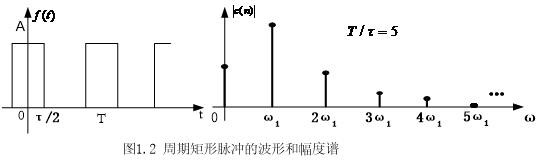
\includegraphics[width=0.8\linewidth]{1-2a.png}
					\caption{周期矩形脉冲的波形和幅度谱}
					\label{fig:周期矩形脉冲的波形和幅度谱}
				\end{figure}

				\begin{figure}[htpb]
					\centering
					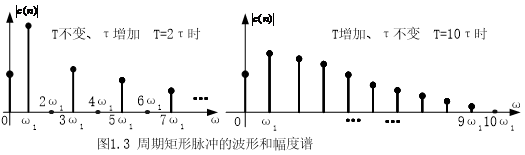
\includegraphics[width=0.8\linewidth]{1-2a2.png}
					\caption{周期矩形脉冲的波形和幅度谱的变化}
					\label{fig:周期矩形脉冲的波形和幅度谱的变化}
				\end{figure}

			\item 三角波的幅度谱如图1.4所示。

				\begin{figure}[htpb]
					\centering
					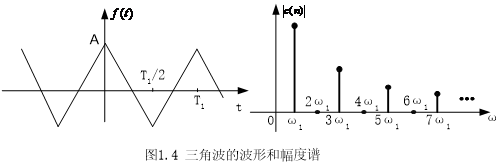
\includegraphics[width=0.8\linewidth]{1-2b.png}
					\caption{三角波的波形和幅度谱}
					\label{fig:三角波的波形和幅度谱}
				\end{figure}

				因此,频谱的测试方法可用频谱分析仪直接测量亦可用逐点测量法进行测量。本实验中使用逐点测量法测量幅度谱。所谓逐点测量法就是按频率由低到高将输入信号的各谐波分量一个一个地测量出来。测量中使用的仪器为选频电平表,选频电平表有两种型号,分别为HX-D21型和YX5014型,其使用方法见附录A。
		\end{enumerate}
\end{enumerate}

\section{实验前预习内容}%
\label{sec:实验前预习内容\arabic{chapter}}

\begin{Exercise}
	计算重复频率为\SI{500}{Hz}的方波、三角波的频谱,并画出频谱图\ref{fig:方波频谱图}、\ref{fig:三角波频谱图}。
\end{Exercise}

\begin{Answer}
	见图\subref{fig:方波频谱图}和\subref{fig:三角波频谱图}。
\end{Answer}

\begin{Exercise}
	计算重复频率为\SI{500}{Hz}、脉冲宽度分别为\SI{0.4}{ms}和\SI{1}{ms}的对称矩形脉冲的频谱,并画出频谱图\ref{fig:对称矩形脉冲频谱图1}、\ref{fig:对称矩形脉冲频谱图2};
\end{Exercise}

\begin{Answer}
	见图\subref{fig:对称矩形脉冲频谱图1}和\subref{fig:对称矩形脉冲频谱图2}。
\end{Answer}

\begin{Exercise}
	利用Matlab画出频率分别为\SI{10}{kHz}与\SI{12}{kHz}的两正弦信号叠加的时域波形图\ref{fig:两正弦波叠加频谱图}。
\end{Exercise}

\begin{Answer}
	见图\subref{fig:两正弦波叠加频谱图}。
\end{Answer}


\langCVfile[Matlab][code:fseries.m][Matlab]{fseries.m}{src/fseries.m}

\langCVfile[Matlab][code:fseriesPlot.m][Matlab]{fseriesPlot.m}{src/fseriesPlot.m}

\langCVfile[Matlab][code:code13.m][Matlab]{code13.m}{src/code13.m}

\begin{figure}[htpb]
	\centering
	\matlablightfile{MATLAB Command Window}{src/code13.txt}
	\caption{运行界面}
	\label{fig:运行界面code13.m}
\end{figure}

\begin{figure}[htpb]
	\centering
	\begin{subfigure}[htpb]{.45\linewidth}
		\centering
		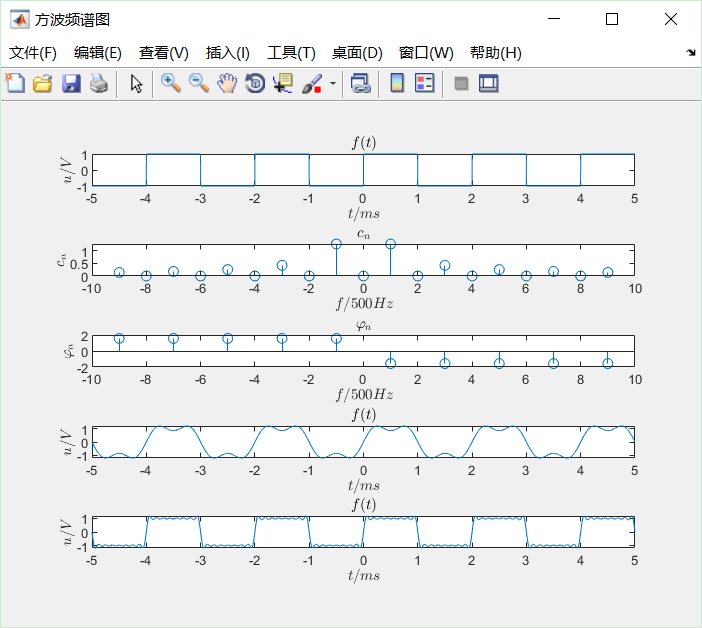
\includegraphics[width=\linewidth]{code131.png}
		\caption{方波频谱图}
		\label{fig:方波频谱图}
	\end{subfigure}
	\quad
	\begin{subfigure}[htpb]{.45\linewidth}
		\centering
		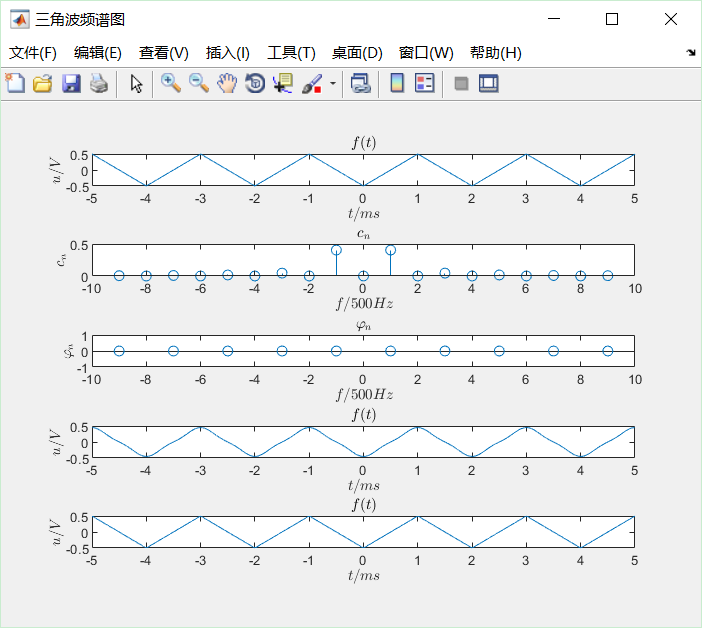
\includegraphics[width=\linewidth]{code132.png}
		\caption{三角波频谱图}
		\label{fig:三角波频谱图}
	\end{subfigure}

	\begin{subfigure}[htpb]{.45\linewidth}
		\centering
		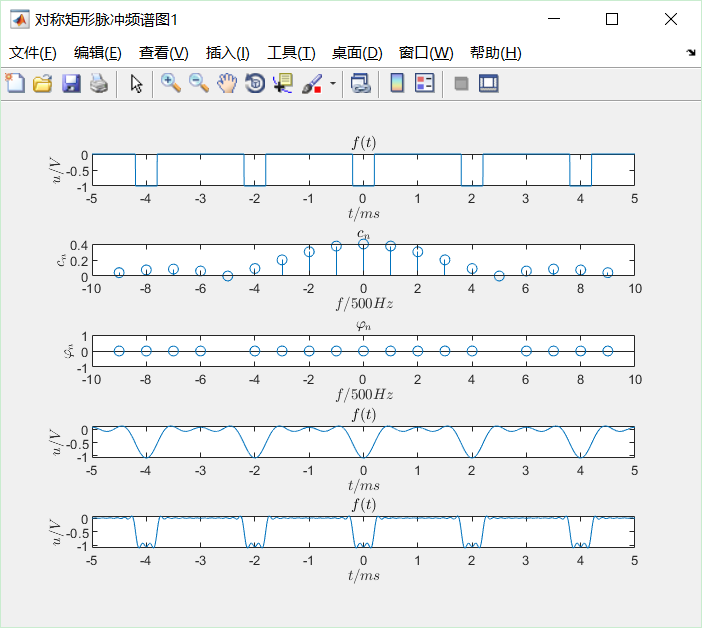
\includegraphics[width=\linewidth]{code133.png}
		\caption{对称矩形脉冲频谱图1}
		\label{fig:对称矩形脉冲频谱图1}
	\end{subfigure}
	\quad
	\begin{subfigure}[htpb]{.45\linewidth}
		\centering
		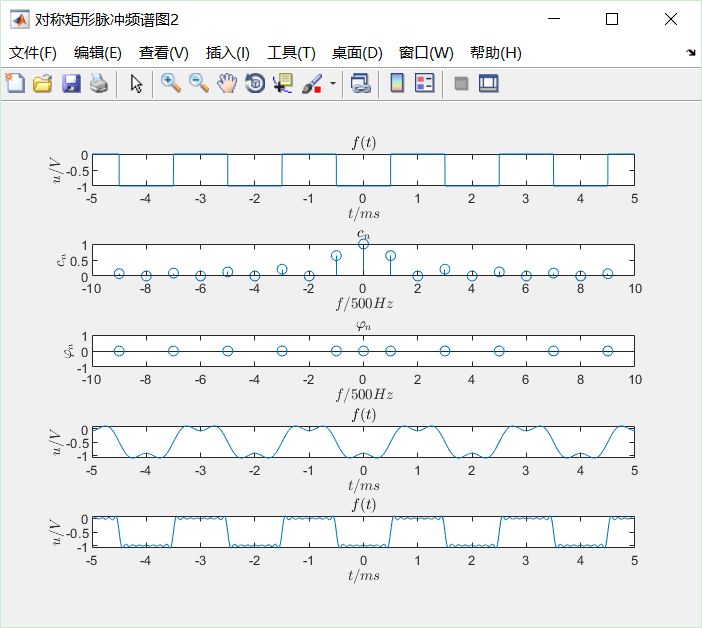
\includegraphics[width=\linewidth]{code134.png}
		\caption{对称矩形脉冲频谱图2}
		\label{fig:对称矩形脉冲频谱图2}
	\end{subfigure}
\end{figure}

\addtocounter{figure}{-1}
\begin{figure}[htpb]
	\centering
	\setcounter{sub}{\value{subfigure}}
	\begin{subfigure}[htpb]{.45\linewidth}
		\setcounter{subfigure}{\value{sub}}
		\centering
		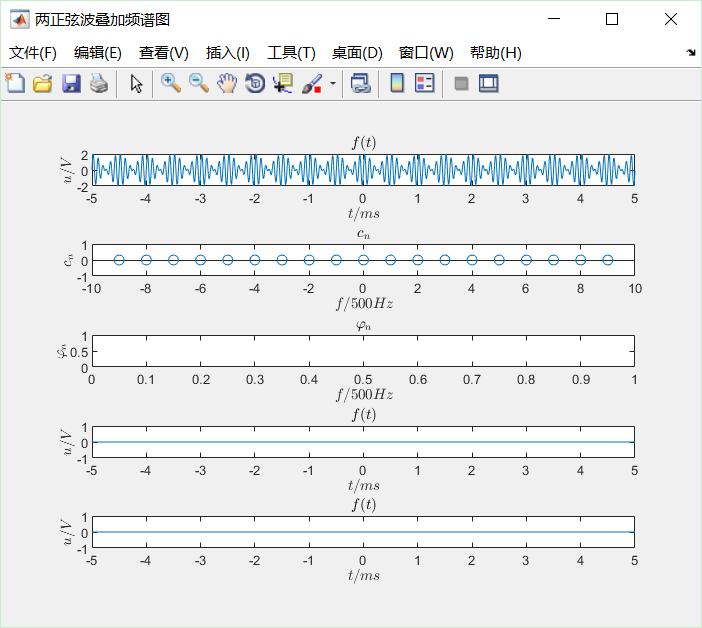
\includegraphics[width=\linewidth]{code135.png}
		\caption{两正弦波叠加频谱图}
		\label{fig:两正弦波叠加频谱图}
	\end{subfigure}
	\caption{频谱图}
	\label{fig:频谱图}
\end{figure}

\newpage

\section{实验原理图}%
\label{sec:实验原理图\arabic{chapter}}

\begin{figure}[htpb]
	\centering
	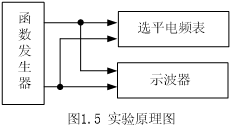
\includegraphics[width=0.6\linewidth]{1-4.png}
	\caption{实验原理图\arabic{chapter}}
	\label{fig:实验原理图\arabic{chapter}}
\end{figure}

\section{实验内容及步骤}%
\label{sec:实验内容及步骤\arabic{chapter}}

\subsection{测试对称方波的频谱}%
\label{sub:测试对称方波的频谱}

将信号源、示波器、选频电平表按图\ref{fig:实验原理图\arabic{chapter}}连接好;信号源输出CH1的输出波形调为方波(P),输出频率调为\SI{500}{Hz},输出信号幅度调为$ V_\text{\text{pp}}=\SI{10}{V} $,按附录A中介绍的选频电平表的使用方法将选频电平表的频率从\SI{200}{Hz}逐渐提高测出方波的前九次谐波分量。测量数据填入表\ref{tab:对称方波的前九次谐波幅度}。

\begin{figure}[htpb]
	\centering
	\begin{subfigure}[htpb]{.45\linewidth}
		\centering
		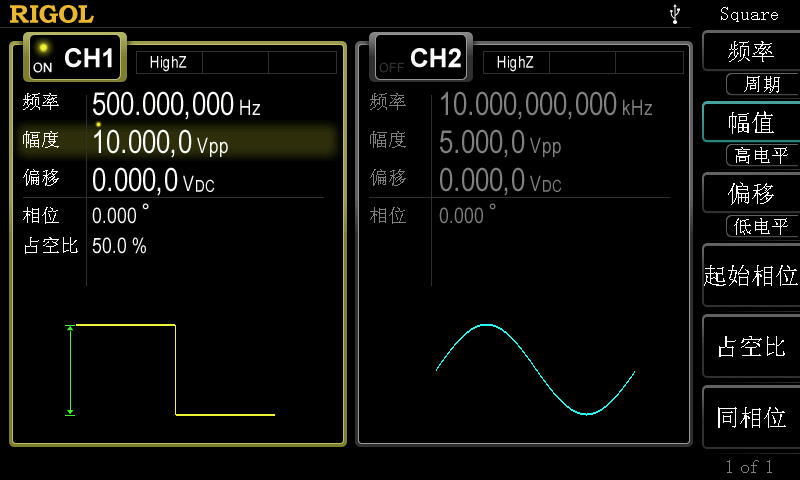
\includegraphics[width=\linewidth]{Rigol11.jpg}
		\caption{信号发生器输出对称方波}
		\label{fig:信号发生器输出对称方波}
	\end{subfigure}
	\quad
	\begin{subfigure}[htpb]{.45\linewidth}
		\centering
		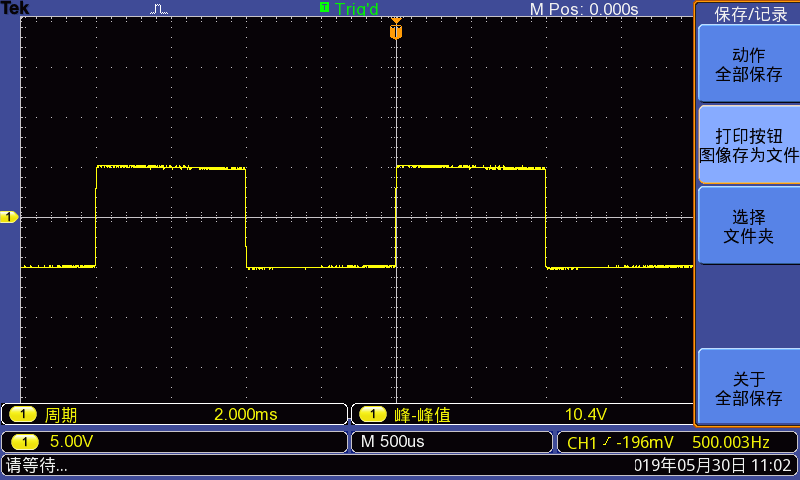
\includegraphics[width=\linewidth]{TEK11.png}
		\caption{示波器测量对称方波}
		\label{fig:示波器测量对称方波}
	\end{subfigure}
	\caption{对称方波}
	\label{fig:对称方波}
\end{figure}

\begin{table}[htpb]
	\centering
	\caption{对称方波的前九次谐波幅度}
	\label{tab:对称方波的前九次谐波幅度}
	\csvreader[
	head to column names,
	tabular=|c|c|c|c|c|c|c|c|c|c|,
	table head=\hline,
	late after line=\\\hline
	]{src/1-5-1.csv}{}{ \a&\b&\c&\d&\e&\f&\g&\h&\i&\j }
\end{table}

\subsection{测试三角波的频谱}%
\label{sub:测试三角波的频谱}

在实验步骤\ref{sub:测试对称方波的频谱}的基础上将信号源输出CH1的输出波形调为三角波(T),频率为\SI{1000}{Hz},幅度为$ V_\text{\text{pp}}=\SI{10}{V} $;用选频电平表测出前九次谐波分量。将测量数据填入表\ref{tab:三角波的前九次谐波幅度}。

\begin{figure}[htpb]
	\centering
	\begin{subfigure}[htpb]{.45\linewidth}
		\centering
		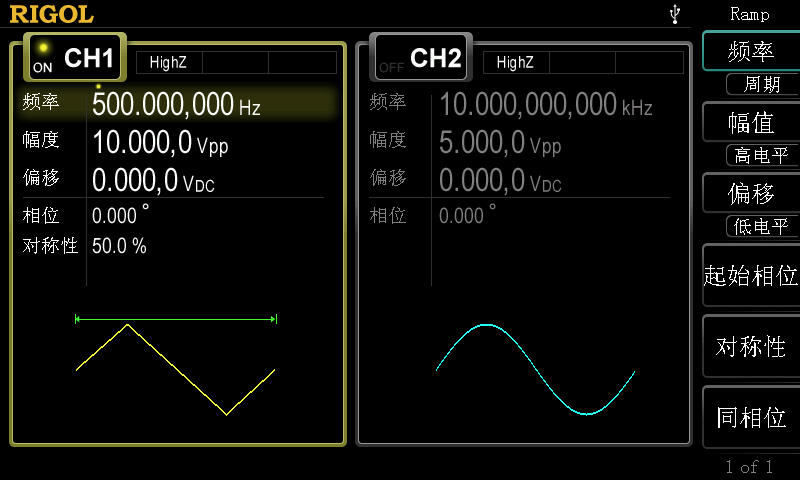
\includegraphics[width=\linewidth]{Rigol12.jpg}
		\caption{信号发生器输出三角波}
		\label{fig:信号发生器输出三角波}
	\end{subfigure}
	\quad
	\begin{subfigure}[htpb]{.45\linewidth}
		\centering
		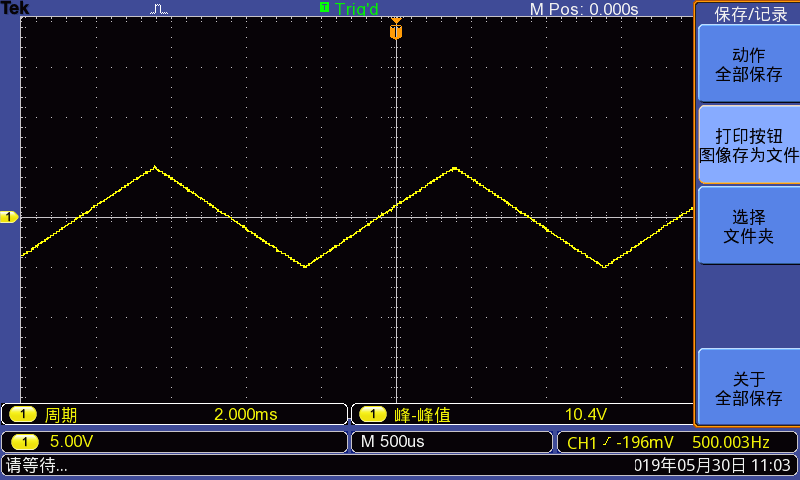
\includegraphics[width=\linewidth]{TEK12.png}
		\caption{示波器测量三角波}
		\label{fig:示波器测量三角波}
	\end{subfigure}
	\caption{三角波}
	\label{fig:三角波}
\end{figure}

\begin{table}[htpb]
	\centering
	\caption{三角波的前九次谐波幅度}
	\label{tab:三角波的前九次谐波幅度}
	\csvreader[
	head to column names,
	tabular=|c|c|c|c|c|c|c|c|c|c|,
	table head=\hline,
	late after line=\\\hline
	]{src/1-5-2.csv}{}{ \a&\b&\c&\d&\e&\f&\g&\h&\i&\j }
\end{table}

\subsection{测试周期矩形脉冲的频谱}%
\label{sub:测试周期矩形脉冲的频谱}

\begin{enumerate}
	\item 将信号源的输出线接“脉冲”输出端 ,信号周期(PP)调为\SI{2}{ms} ,脉宽(PW)调为\SI{0.4}{ms},用选频电平表测出信号的前九次谐波分量,填入表\ref{tab:周期矩形脉冲的前九次谐波幅度\arabic{enumi}}。

		\begin{figure}[htpb]
			\centering
			\begin{subfigure}[htpb]{.45\linewidth}
				\centering
				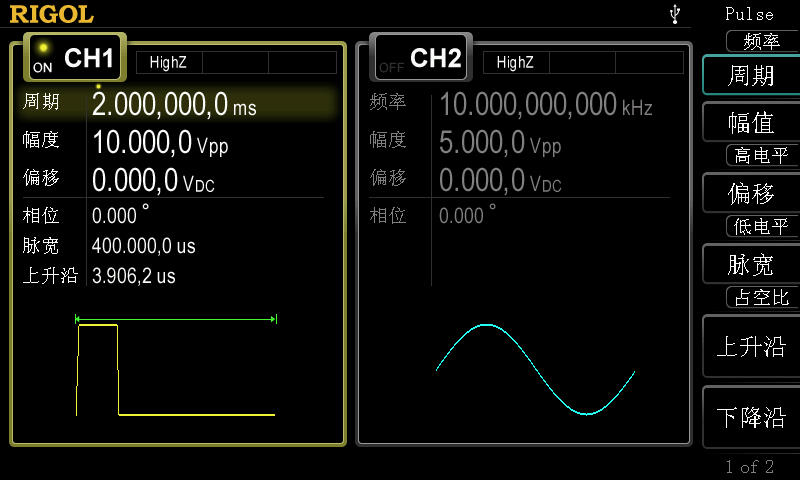
\includegraphics[width=\linewidth]{Rigol131.jpg}
				\caption{信号发生器输出周期矩形脉冲\arabic{enumi}}
				\label{fig:信号发生器输出周期矩形脉冲\arabic{enumi}}
			\end{subfigure}
			\quad
			\begin{subfigure}[htpb]{.45\linewidth}
				\centering
				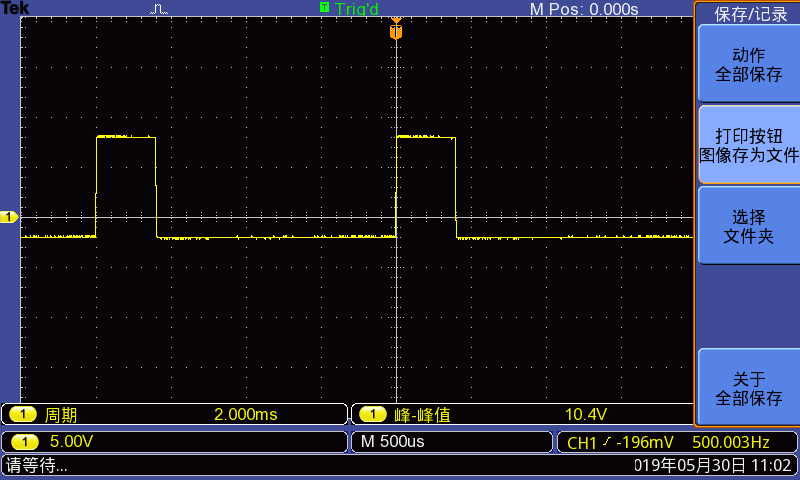
\includegraphics[width=\linewidth]{TEK131.png}
				\caption{示波器测量周期矩形脉冲\arabic{enumi}}
				\label{fig:示波器测量周期矩形脉冲\arabic{enumi}}
			\end{subfigure}
			\caption{周期矩形脉冲\arabic{enumi}}
			\label{fig:周期矩形脉冲\arabic{enumi}}
		\end{figure}

		\begin{table}[htpb]
			\centering
			\caption{周期矩形脉冲的前九次谐波幅度\arabic{enumi}}
			\label{tab:周期矩形脉冲的前九次谐波幅度\arabic{enumi}}
			\csvreader[
			head to column names,
			tabular=|c|c|c|c|c|c|c|c|c|c|,
			table head=\hline,
			late after line=\\\hline
			]{src/1-5-3.csv}{}{ \a&\b&\c&\d&\e&\f&\g&\h&\i&\j }
		\end{table}

	\item 将信号的脉宽(PW)调为\SI{1}{ms},周期保持不变,测出其前九次谐波分量,填入表\ref{tab:周期矩形脉冲的前九次谐波幅度\arabic{enumi}},并与内容\ref{sub:测试对称方波的频谱}进行比较。

		\begin{figure}[htpb]
			\centering
			\begin{subfigure}[htpb]{.45\linewidth}
				\centering
				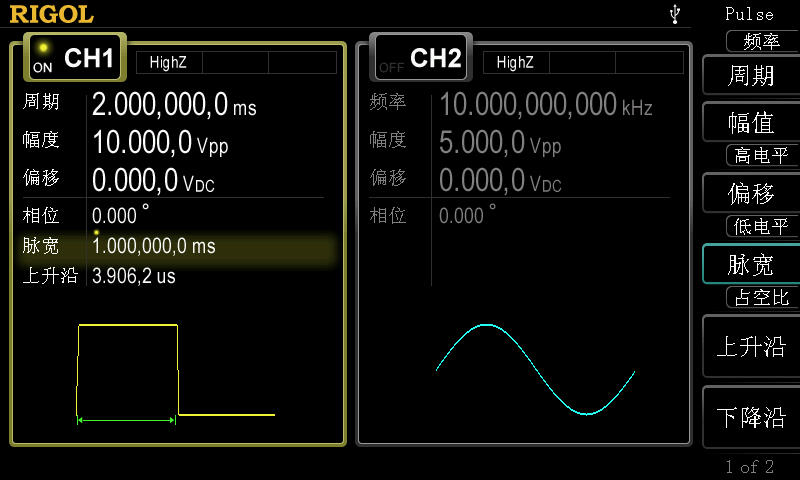
\includegraphics[width=\linewidth]{Rigol132.jpg}
				\caption{信号发生器输出周期矩形脉冲\arabic{enumi}}
				\label{fig:信号发生器输出周期矩形脉冲\arabic{enumi}}
			\end{subfigure}
			\quad
			\begin{subfigure}[htpb]{.45\linewidth}
				\centering
				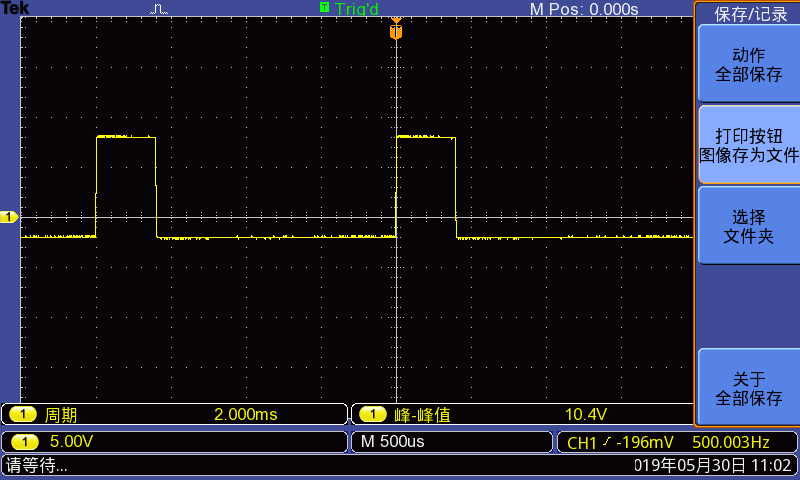
\includegraphics[width=\linewidth]{TEK131.png}
				\caption{示波器测量周期矩形脉冲\arabic{enumi}}
				\label{fig:示波器测量周期矩形脉冲\arabic{enumi}}
			\end{subfigure}
			\caption{周期矩形脉冲\arabic{enumi}}
			\label{fig:周期矩形脉冲\arabic{enumi}}
		\end{figure}

		\begin{table}[htpb]
			\centering
			\caption{周期矩形脉冲的前九次谐波幅度\arabic{enumi}}
			\label{tab:周期矩形脉冲的前九次谐波幅度\arabic{enumi}}
			\csvreader[
			head to column names,
			tabular=|c|c|c|c|c|c|c|c|c|c|,
			table head=\hline,
			late after line=\\\hline
			]{src/1-5-3a.csv}{}{ \a&\b&\c&\d&\e&\f&\g&\h&\i&\j }
		\end{table}
\end{enumerate}

\subsection{观测两正弦信号叠加后的波形及频谱}%
\label{sub:观测两正弦信号叠加后的波形及频谱}

将信号源按图\ref{fig:正弦信号叠加的原理图}所示连接好,并将输出波形均调为正弦波(S);

\begin{figure}[htpb]
	\centering
	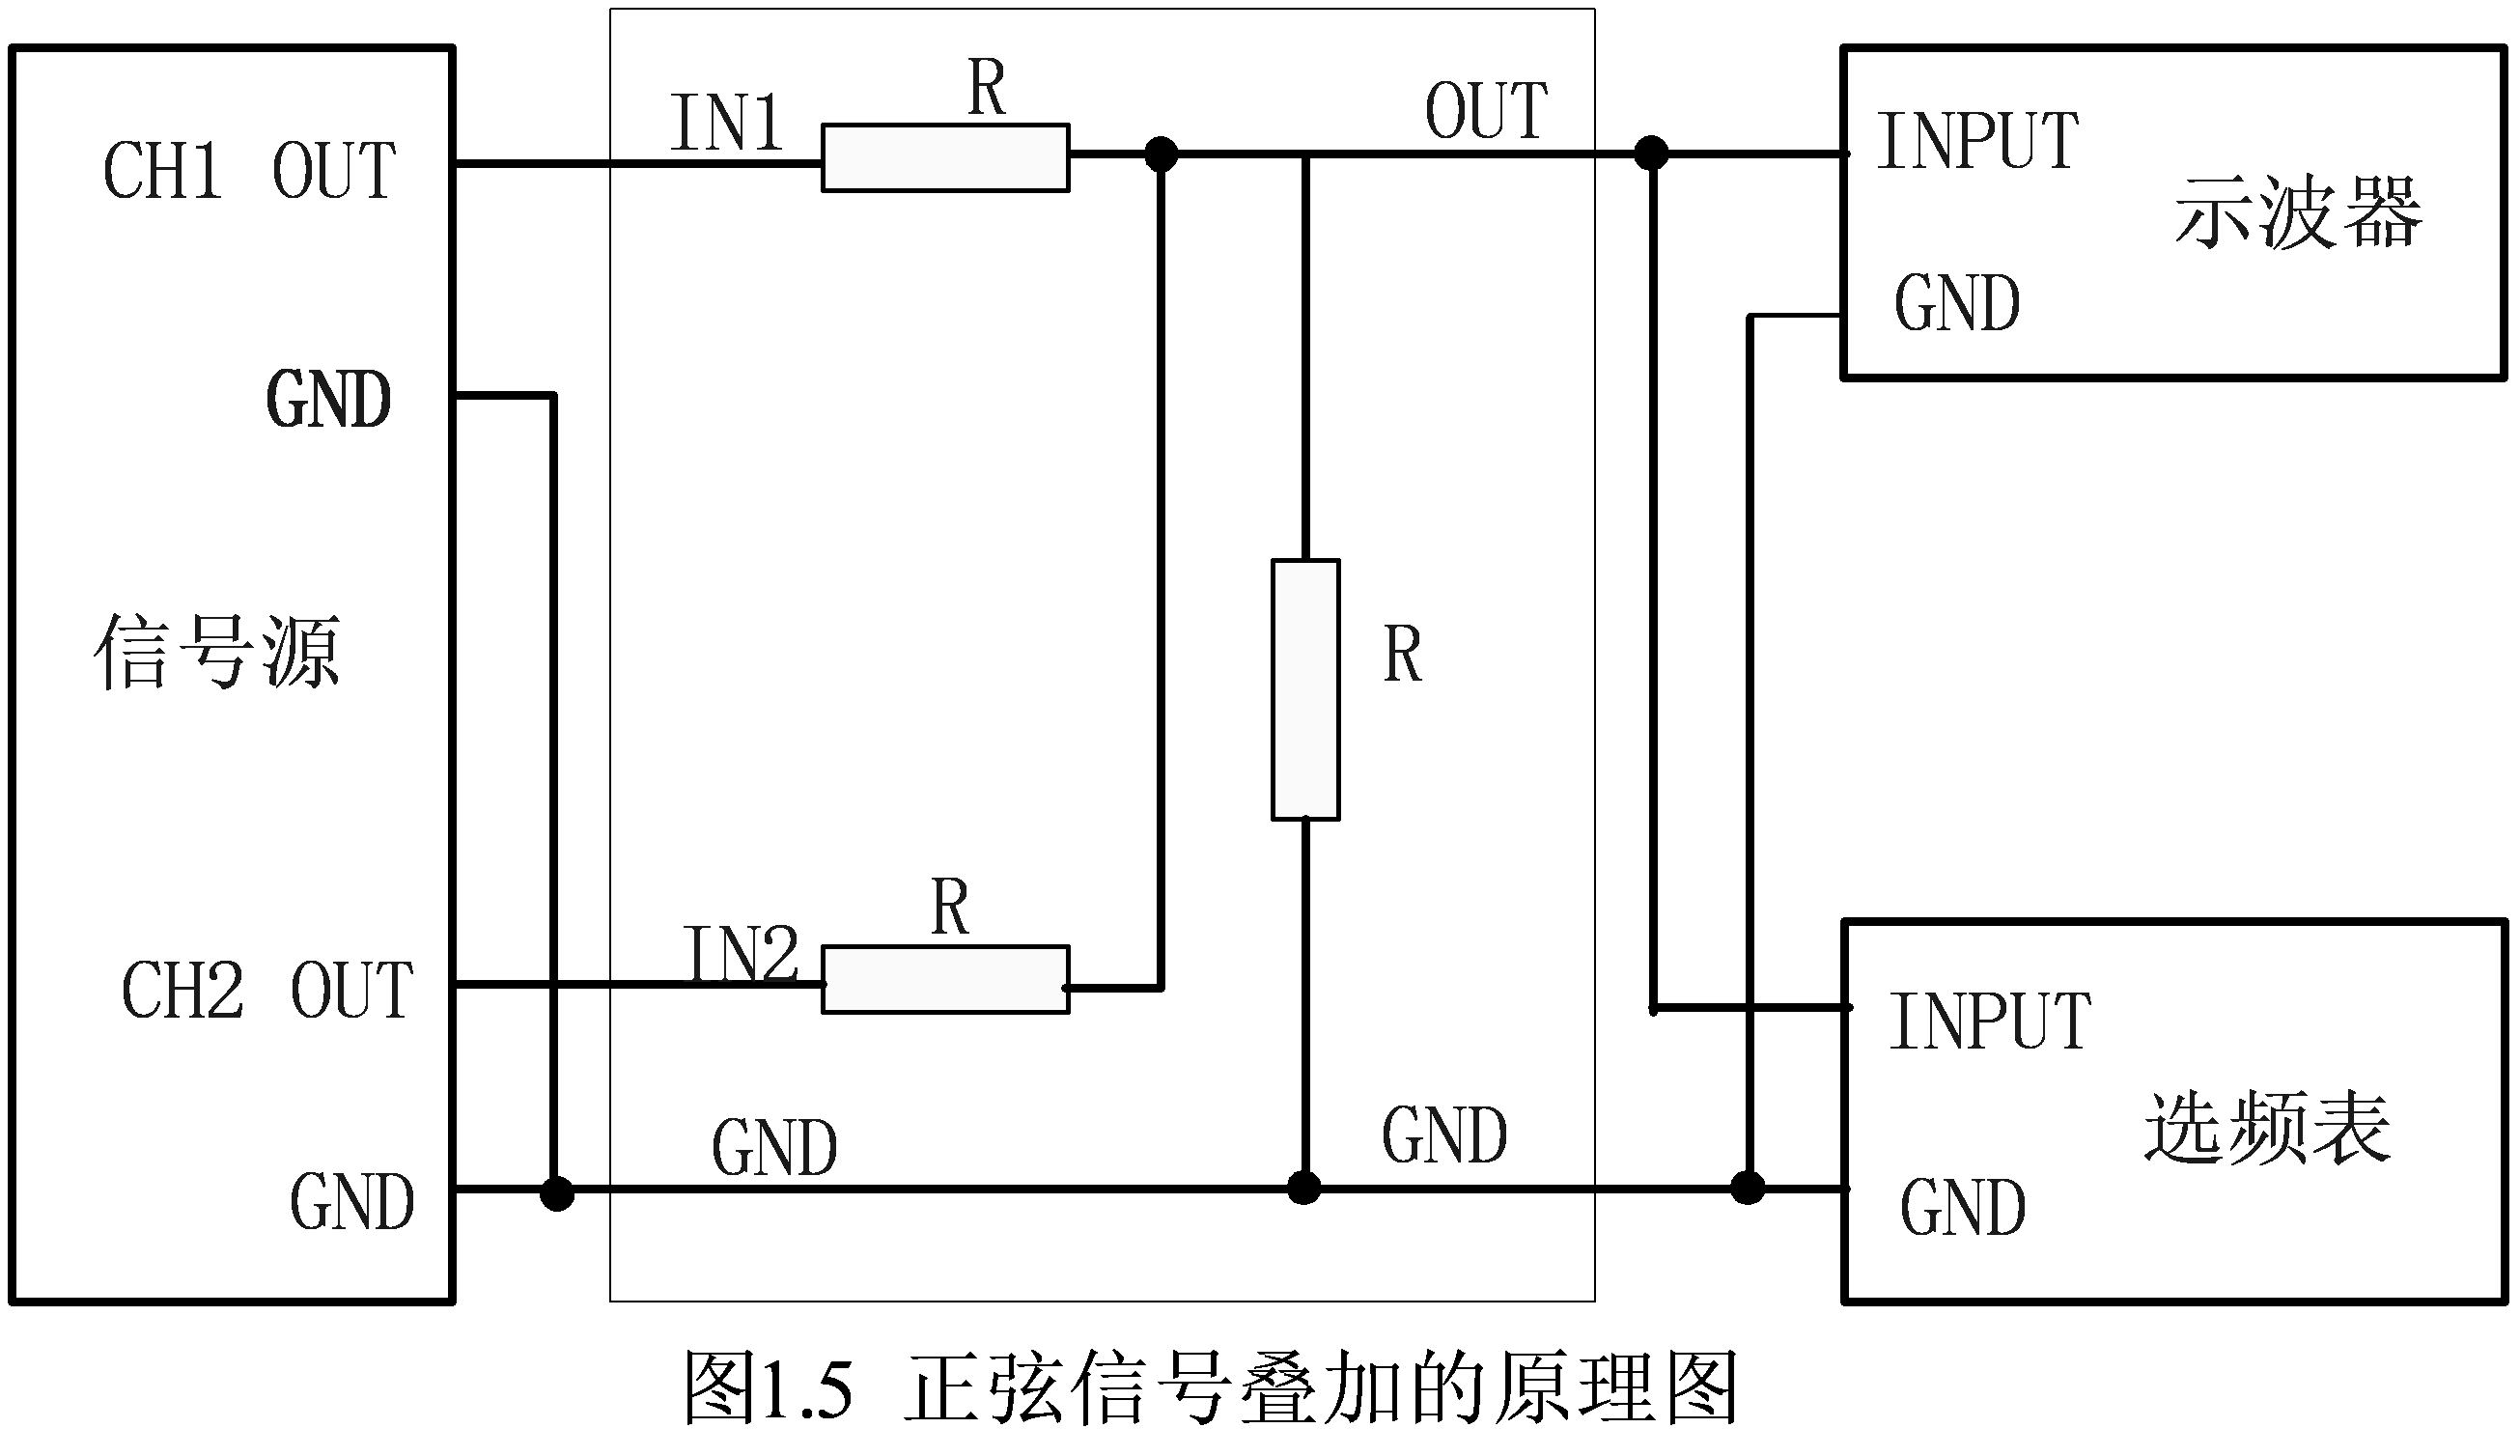
\includegraphics[width=0.6\linewidth]{1-5-4.png}
	\caption{正弦信号叠加的原理图}
	\label{fig:正弦信号叠加的原理图}
\end{figure}

\begin{enumerate}
	\item 再将信号源两路(CH1,CH2)的频率差距加大,即分别调为\SI{500}{Hz}和\SI{10}{kHz},幅度仍为$ V_{\text{pp}}=\SI{5}{V} $,观测示波器上的输出波形并记录,然后测出其频谱表\ref{tab:正弦信号叠加的频谱\arabic{enumi}},记录测量数据。

		\begin{table}[htpb]
			\centering
			\caption{正弦信号叠加的频谱\arabic{enumi}}
			\label{tab:正弦信号叠加的频谱\arabic{enumi}}
			\csvreader[
			head to column names,
			tabular=|c|c|c|,
			table head=\hline,
			late after line=\\\hline
			]{src/1-5-4.csv}{}{ \a&\b&\c }
		\end{table}

		\begin{figure}[htpb]
			\centering
			\begin{subfigure}[htpb]{.45\linewidth}
				\centering
				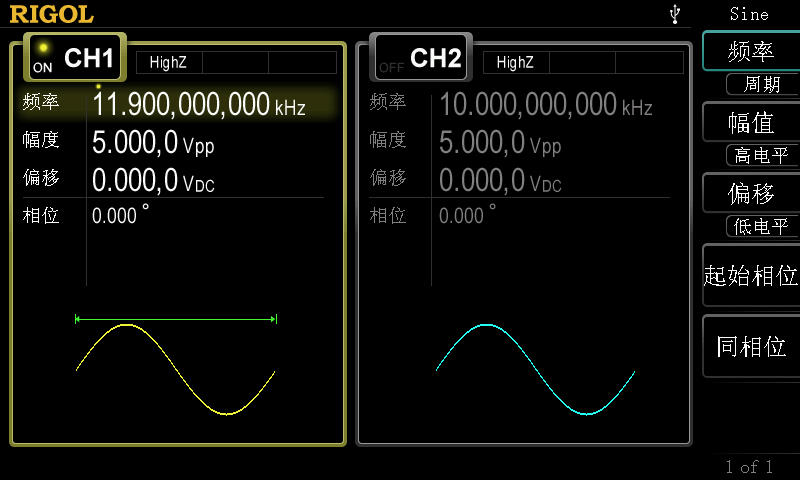
\includegraphics[width=\linewidth]{Rigol142.jpg}
				\caption{函数发生器输出两正弦信号叠加后的波形\arabic{enumi}}
				\label{fig:函数发生器输出两正弦信号叠加后的波形\arabic{enumi}}
			\end{subfigure}
			\quad
			\begin{subfigure}[htpb]{.45\linewidth}
				\centering
				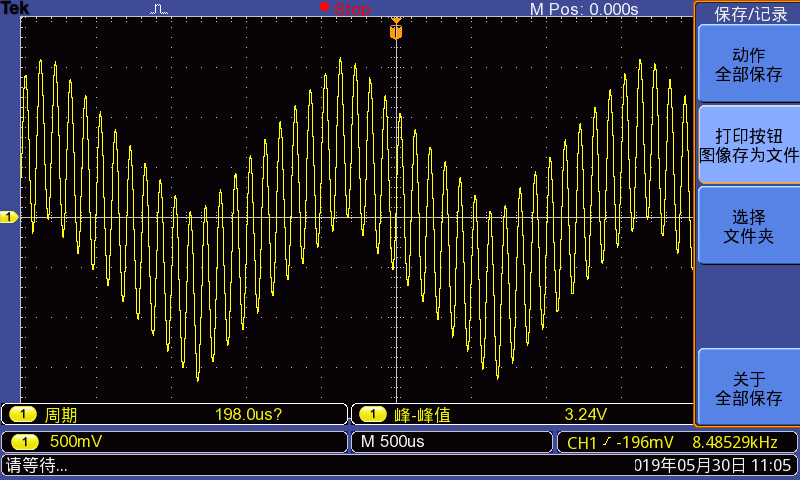
\includegraphics[width=\linewidth]{TEK141.png}
				\caption{示波器测量两正弦信号叠加后的波形\arabic{enumi}}
				\label{fig:示波器测量两正弦信号叠加后的波形\arabic{enumi}}
			\end{subfigure}
			\caption{两正弦信号叠加后的波形\arabic{enumi}}
			\label{fig:两正弦信号叠加后的波形\arabic{enumi}}
		\end{figure}

	\item 将信号源两路输出(CH1,CH2)的频率分别调为\SI{10}{kHz}和\SI{11.9}{kHz},信号幅度均调为$ V_\text{pp}=\SI{5}{V} $,观测示波器上的输出波形并定性记录,然后测出其频谱表\ref{tab:正弦信号叠加的频谱\arabic{enumi}},记录测量数据。

		\begin{figure}[htpb]
			\centering
			\begin{subfigure}[htpb]{.45\linewidth}
				\centering
				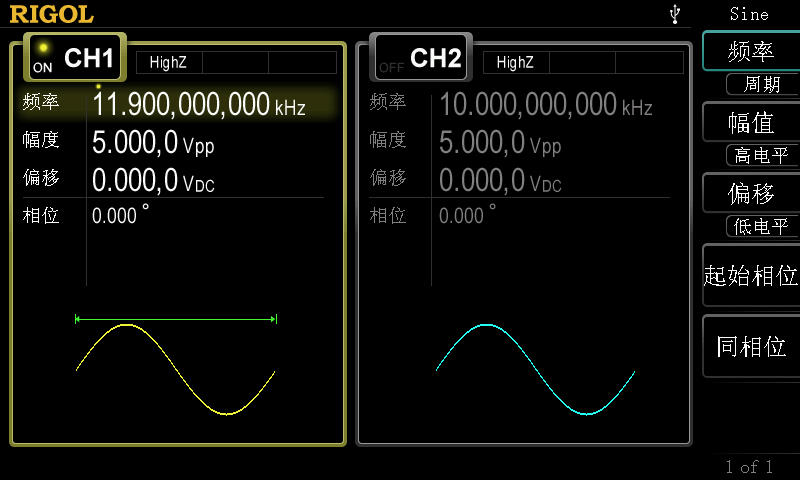
\includegraphics[width=\linewidth]{Rigol142.jpg}
				\caption{函数发生器输出两正弦信号叠加后的波形\arabic{enumi}}
				\label{fig:函数发生器输出两正弦信号叠加后的波形\arabic{enumi}}
			\end{subfigure}
			\quad
			\begin{subfigure}[htpb]{.45\linewidth}
				\centering
				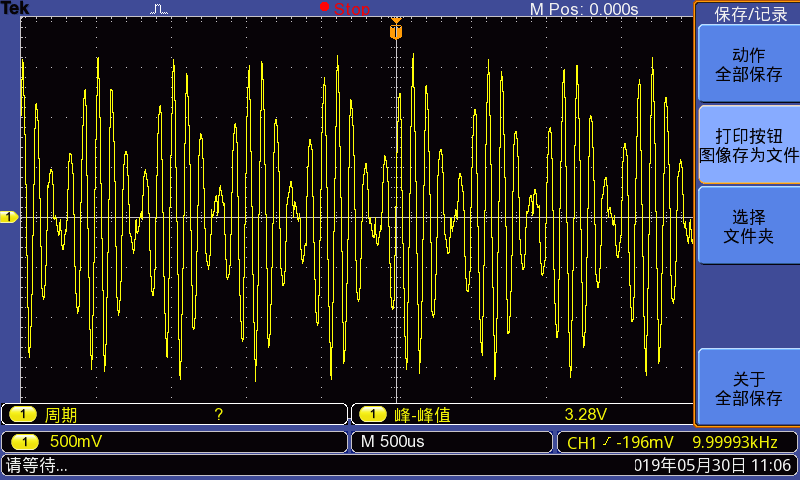
\includegraphics[width=\linewidth]{TEK142.png}
				\caption{示波器测量两正弦信号叠加后的波形\arabic{enumi}}
				\label{fig:示波器测量两正弦信号叠加后的波形\arabic{enumi}}
			\end{subfigure}
			\caption{两正弦信号叠加后的波形\arabic{enumi}}
			\label{fig:两正弦信号叠加后的波形\arabic{enumi}}
		\end{figure}

		\begin{table}[htpb]
			\centering
			\caption{正弦信号叠加的频谱\arabic{enumi}}
			\label{tab:正弦信号叠加的频谱\arabic{enumi}}
			\csvreader[
			head to column names,
			tabular=|c|c|c|,
			table head=\hline,
			late after line=\\\hline
			]{src/1-5-4a.csv}{}{ \a&\b&\c }
		\end{table}
\end{enumerate}

\section{实验仪器及设备}%
\label{sec:实验仪器及设备\arabic{chapter}}

双踪示波器一台,函数发生器一台,选频电平表一台,  实验板一块。

\section{实验报告要求}%
\label{sec:实验报告要求\arabic{chapter}}

\begin{Exercise}
	叙述实验内容及实验步骤。
\end{Exercise}

\begin{Answer}
	实验内容及步骤见第\ref{sec:实验内容及步骤\arabic{chapter}}节。
\end{Answer}

\begin{Exercise}
	整理实验数据,并根据实验数据画出频谱图。
\end{Exercise}

\begin{Answer}
	实验数据见表\ref{tab:对称方波的前九次谐波幅度}、\ref{tab:三角波的前九次谐波幅度}、\ref{tab:周期矩形脉冲的前九次谐波幅度1}、\ref{tab:周期矩形脉冲的前九次谐波幅度2}、\ref{tab:正弦信号叠加的频谱1}和\ref{tab:正弦信号叠加的频谱2}。频谱图见图\ref{fig:对称方波}、\ref{fig:三角波}、\ref{fig:周期矩形脉冲1}、\ref{fig:周期矩形脉冲2}、\ref{fig:两正弦信号叠加后的波形1}和\ref{fig:两正弦信号叠加后的波形2}。
\end{Answer}

\begin{Exercise}
	对实验内容\ref{sub:测试周期矩形脉冲的频谱}的实验数据进行分析并给出结论。
\end{Exercise}

\begin{Answer}
	当$ T $不变$ \tau $增加时幅度增加,间隔增加;当$ \tau $不变$ T $增加时幅度减小,间隔减小。
\end{Answer}

\begin{Exercise}
	画出实验中观测到的正弦信号叠加的波形,并将实验波形与仿真波形进行比较。
\end{Exercise}

\begin{Answer}
	观测波形见图\ref{fig:两正弦信号叠加后的波形1}和\ref{fig:两正弦信号叠加后的波形2},波形见图\ref{fig:两正弦波叠加频谱图},比较后发现仿真结果和实验比较吻合。
\end{Answer}

\begin{Exercise}
	说明不同频率正弦信号叠加后信号的特点。
\end{Exercise}

\begin{Answer}
	叠加后波形的形状与各信号的频率、初相、幅值有关,虽然不再是正弦信号,但一定是周期信号,且周期与最低频率分量的信号周期相同。
\end{Answer}


\chapter{系统频率响应特性的测量}%
\label{cha:系统频率响应特性的测量}
\section{实验目的}%
\label{sec:实验目的\arabic{chapter}}
\begin{enumerate}
	\item 掌握频率响应特性的测量方法;
	\item 研究典型网络的频率响应特性。
\end{enumerate}
\section{实验原理及方法}%
\label{sec:实验原理及方法\arabic{chapter}}
\begin{enumerate}
	\item 系统的频率响应特性是指系统在正弦信号激励下系统的稳态响应随激励信号频率变化的情况。用矢量形式表示:
		\begin{align}
			H(\jmath\Omega) = \frac{Y(\jmath\Omega)}{X(\jmath\Omega)} = |H(\jmath\Omega)| \text{e}^{\jmath\varphi(\Omega)}
		\end{align}
		其中:$ |H(\jmath\Omega)| $为幅频特性,表示输出信号与输入信号的幅度比随输入信号频率的变化关系;$ \varphi(\Omega) $为相频特性,表示输出信号与输入信号的相位差随输入信号频率的变化关系。
	\item $ H(\jmath\Omega) $可根据系统函数$ H(s) $求得:
		\begin{align}
			H(\jmath\Omega)=H(s)\Big|_{s=\jmath\Omega}
		\end{align}
		因此,对于给定的电路可根椐$ s $域模型先求出系统函数$ H(s) $,再求$ H(\jmath\Omega) $,然后讨论系统的频响特性。
	\item 频响特性的测量可分别测量幅频特性和相频特性,幅频特性的测试采用改变激励信号的频率逐点测出响应的幅度,然后用描图法描出幅频特性曲线;相频特性的测量方法亦可改变激励信号的频率用双踪示波器逐点测出输出信号与输入信号的延时$ \tau $,根椐下面的公式推算出相位差$ \varphi(\Omega) $。
		\begin{align}
			\varphi(\Omega)=2\pi\times \frac{\tau}{T}
		\end{align}
		当响应超前激励时$ \varphi(\Omega) $为正,当响应落后激励时$ \varphi(\Omega) $为负。
\end{enumerate}
\section{实验前预习内容}%
\label{sec:实验前预习内容\arabic{chapter}}
\begin{Exercise}
	写出原理图中高、低通及并联后滤波器网络的电压转移函数。
\end{Exercise}
\begin{Answer}
	\begin{align}
		H_\text{HP}(s)&=\dfrac{\dfrac{R}{2}}{\dfrac{R}{2}+\dfrac{1}{sC}}
		\\
		H_\text{LP}(s)&=\dfrac{\dfrac{1}{2sC}}{\dfrac{1}{2sC}+R}
		\\
		H_\text{BS}(s)&=\dfrac{\dfrac{R}{2}}{\dfrac{R}{2}+\dfrac{1}{sC}}+\dfrac{\dfrac{1}{2sC}}{\dfrac{1}{2sC}+R}
	\end{align}
\end{Answer}
\begin{Exercise}
	利用Matlab画出图中高、低通及并联后滤波器网络的幅频特性及相频特性曲线,并计算截止频率。
\end{Exercise}
\begin{Answer}
	频响特性曲线见图\subref{fig:高通滤波器频响特性曲线}、\subref{fig:低通滤波器频响特性曲线}和\subref{fig:带通滤波器频响特性曲线}。截止频率见\ref{fig:运行界面code232.m}。
\end{Answer}
\langCVfile[Matlab][code:freqPlot.m][Matlab]{freqPlot.m}{src/freqPlot.m}
\langCVfile[Matlab][code:code232.m][Matlab]{code232.m}{src/code232.m}
\begin{figure}[htpb]
	\centering
	\matlablightfile{MATLAB Command Window}{src/code232.txt}
	\caption{运行界面}
	\label{fig:运行界面code232.m}
\end{figure}
\begin{figure}[htpb]
	\centering
	\begin{subfigure}[htpb]{.45\linewidth}
		\centering
		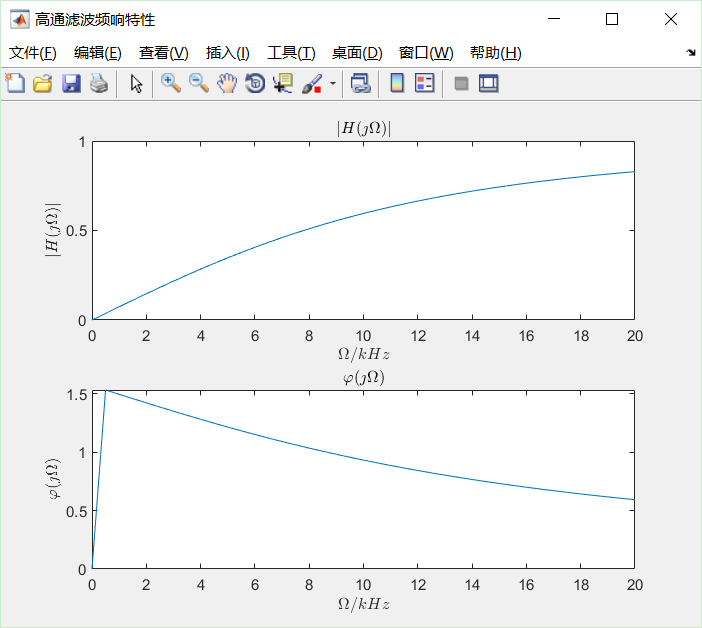
\includegraphics[width=\linewidth]{HP.png}
		\caption{高通滤波器频响特性曲线}
		\label{fig:高通滤波器频响特性曲线}
	\end{subfigure}
	\quad
	\begin{subfigure}[htpb]{.45\linewidth}
		\centering
		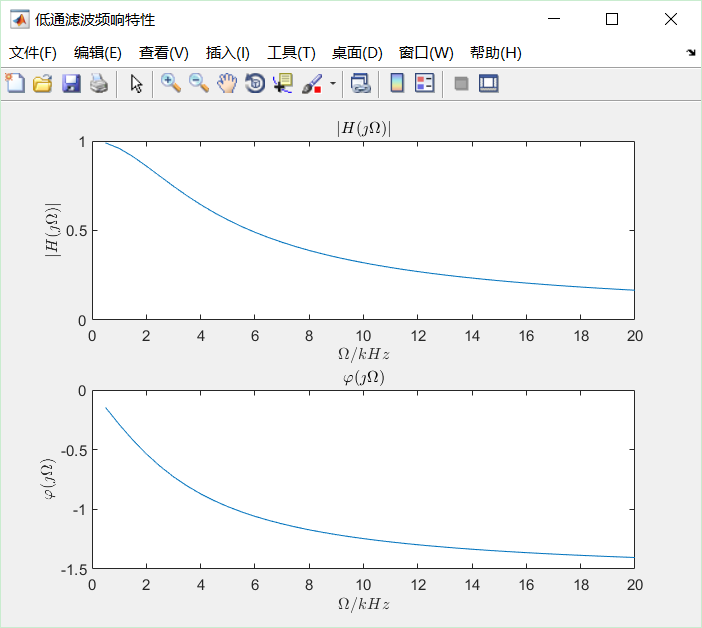
\includegraphics[width=\linewidth]{LP.png}
		\caption{低通滤波器频响特性曲线}
		\label{fig:低通滤波器频响特性曲线}
	\end{subfigure}
	\begin{subfigure}[htpb]{.45\linewidth}
		\centering
		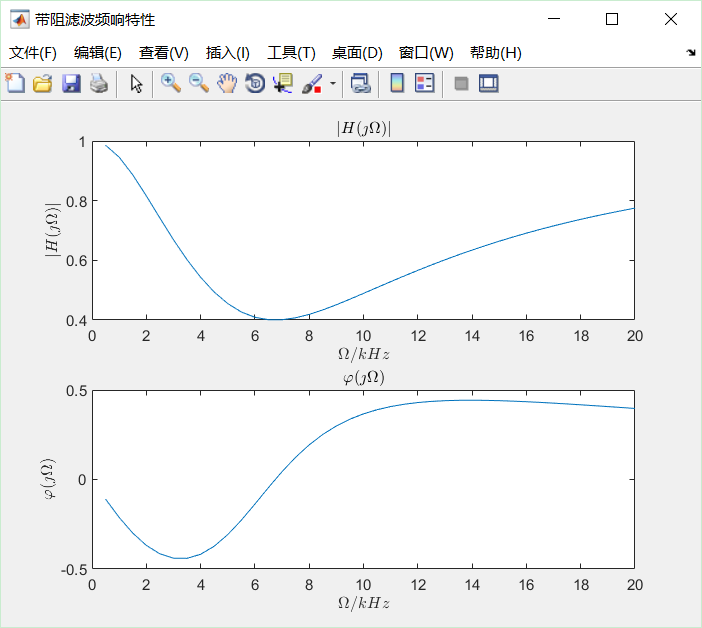
\includegraphics[width=\linewidth]{BS.png}
		\caption{带通滤波器频响特性曲线}
		\label{fig:带通滤波器频响特性曲线}
	\end{subfigure}
	\caption{频响特性曲线}
	\label{fig:频响特性曲线}
\end{figure}
\begin{Exercise}
	思考测量输入、输出信号相位差的具体方法。
\end{Exercise}
\begin{Answer}
	通过在双踪示波器器上测量。
\end{Answer}
\begin{Exercise}
	思考测试频率特性时,测试点频率应如何选取。
\end{Exercise}
\begin{Answer}
	测试点应在截止频率附近多选。
\end{Answer}
\section{实验原理图}%
\label{sec:实验原理图\arabic{chapter}}
\begin{figure}[htpb]
	\centering
	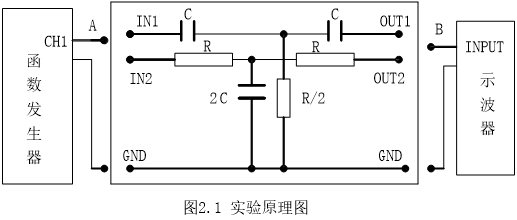
\includegraphics[width=0.8\linewidth]{2-4.png}
	\caption{实验原理图\arabic{chapter}}
	\label{fig:实验原理图\arabic{chapter}}
\end{figure}
图中:$ R=\SI{38}{k\ohm} $,$ C=\SI{3900}{pF} $,方框内为实验板上的电路。
\section{实验内容及步骤}%
\label{sec:实验内容及步骤\arabic{chapter}}
将信号源输出CH1的信号波形调为正弦波,信号的幅度调为$ V_\text{pp}=\SI{10}{V} $。
\subsection{RC高通滤波器的频响特性的测量}%
\label{sub:RC高通滤波器的频响特性的测量}
将信号源的输出端(A)接实验板的IN1端,滤波后的信号OUT1接示波器的输入(B) 。根据被测电路的参数及系统的频特性,将输入信号的频率从低到高逐次改变十 次以上(幅度保持$ V_\text{ipp}=\SI{10}{V} $) , 逐个测量输出信号的峰峰值大小($ V_\text{opp} $)及输出信号与输入信号的相位差 ,并将测量数据填入表\ref{tab:RC高通滤波器测量数据}:
\begin{figure}[htpb]
	\centering
	\begin{subfigure}[htpb]{.45\linewidth}
		\centering
		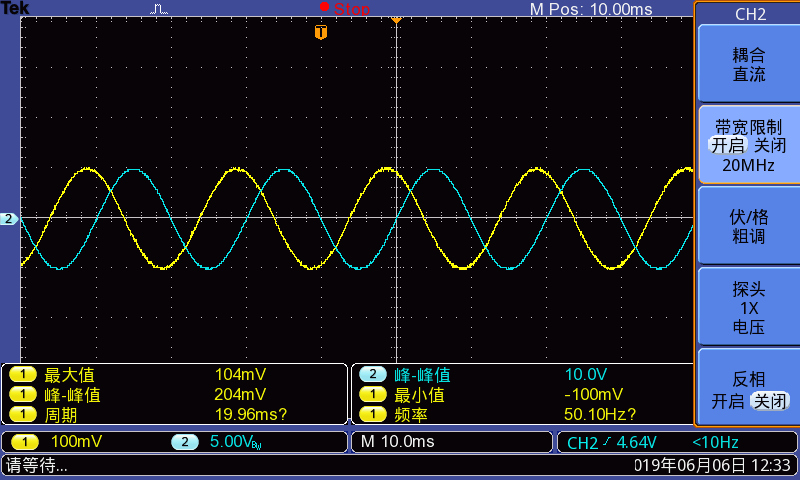
\includegraphics[width=\linewidth]{TEK21.png}
		\caption{RC高通滤波器测量数据\arabic{subfigure}}
		\label{fig:RC高通滤波器测量数据\arabic{subfigure}}
	\end{subfigure}
	\quad
	\begin{subfigure}[htpb]{.45\linewidth}
		\centering
		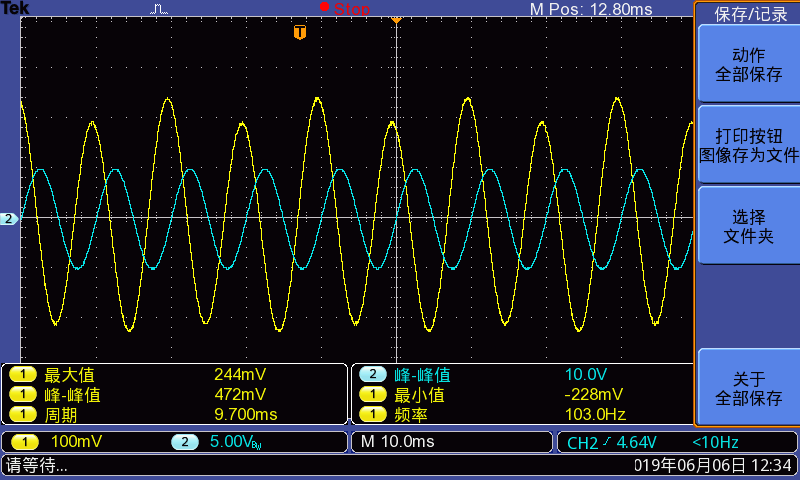
\includegraphics[width=\linewidth]{TEK22.png}
		\caption{RC高通滤波器测量数据\arabic{subfigure}}
		\label{fig:RC高通滤波器测量数据\arabic{subfigure}}
	\end{subfigure}
	\begin{subfigure}[htpb]{.45\linewidth}
		\centering
		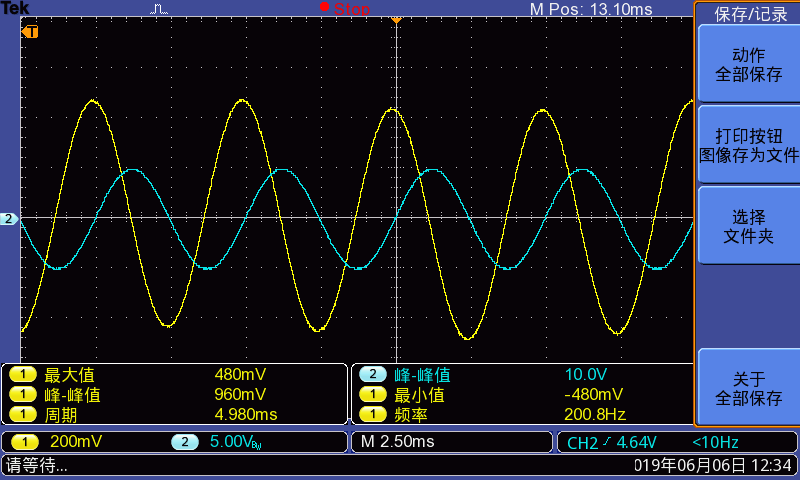
\includegraphics[width=\linewidth]{TEK23.png}
		\caption{RC高通滤波器测量数据\arabic{subfigure}}
		\label{fig:RC高通滤波器测量数据\arabic{subfigure}}
	\end{subfigure}
	\quad
	\begin{subfigure}[htpb]{.45\linewidth}
		\centering
		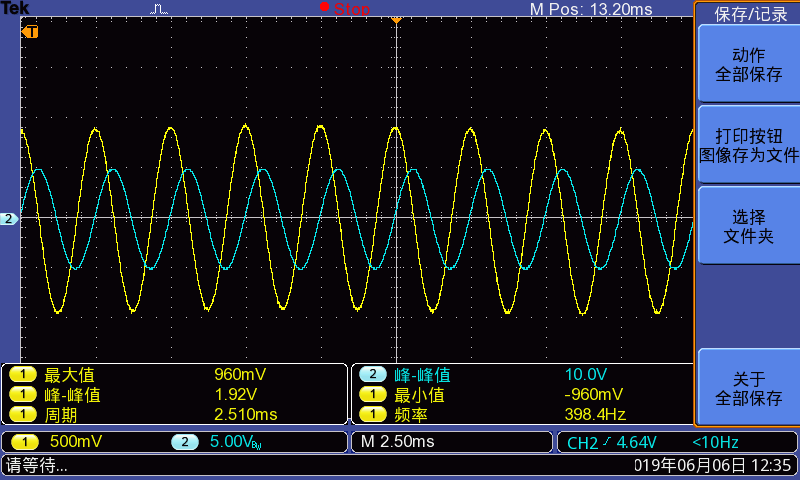
\includegraphics[width=\linewidth]{TEK24.png}
		\caption{RC高通滤波器测量数据\arabic{subfigure}}
		\label{fig:RC高通滤波器测量数据\arabic{subfigure}}
	\end{subfigure}
	\begin{subfigure}[htpb]{.45\linewidth}
		\centering
		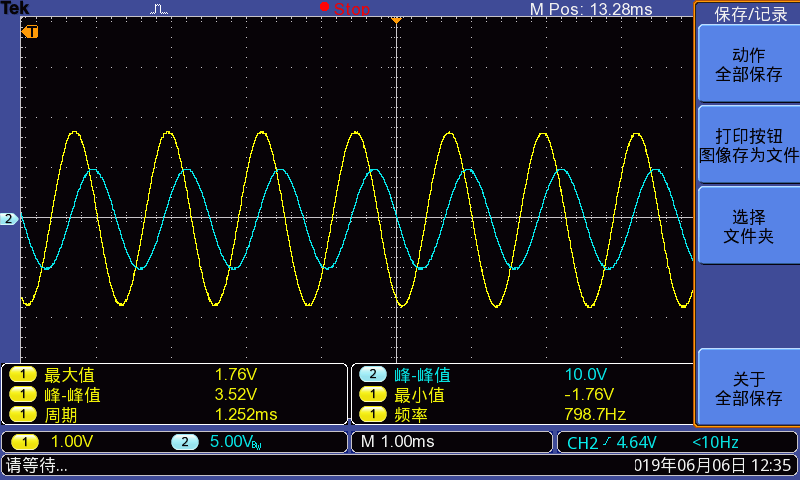
\includegraphics[width=\linewidth]{TEK25.png}
		\caption{RC高通滤波器测量数据\arabic{subfigure}}
		\label{fig:RC高通滤波器测量数据\arabic{subfigure}}
	\end{subfigure}
	\quad
	\begin{subfigure}[htpb]{.45\linewidth}
		\centering
		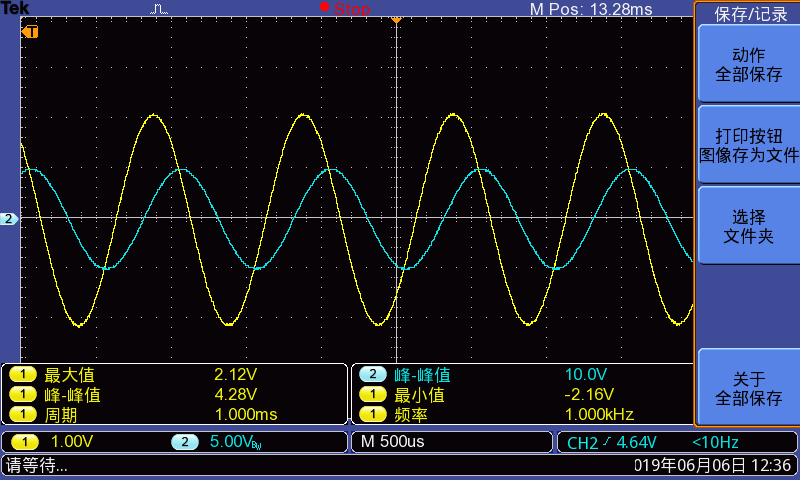
\includegraphics[width=\linewidth]{TEK26.png}
		\caption{RC高通滤波器测量数据\arabic{subfigure}}
		\label{fig:RC高通滤波器测量数据\arabic{subfigure}}
	\end{subfigure}
	\begin{subfigure}[htpb]{.45\linewidth}
		\centering
		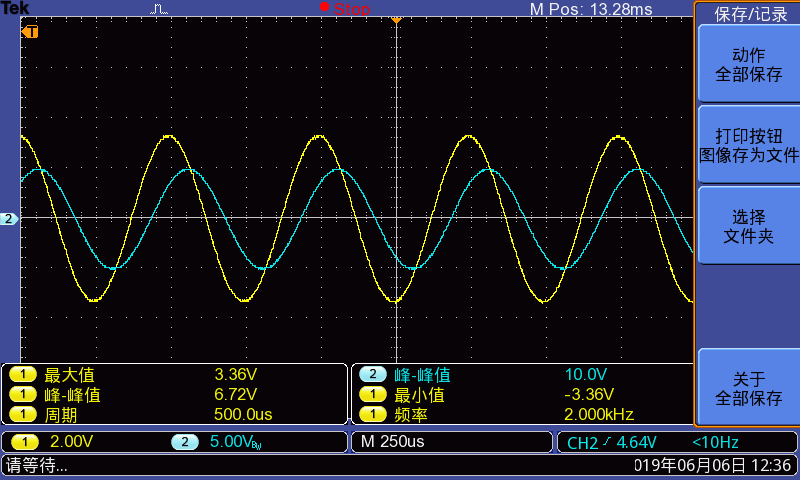
\includegraphics[width=\linewidth]{TEK27.png}
		\caption{RC高通滤波器测量数据\arabic{subfigure}}
		\label{fig:RC高通滤波器测量数据\arabic{subfigure}}
	\end{subfigure}
	\quad
	\begin{subfigure}[htpb]{.45\linewidth}
		\centering
		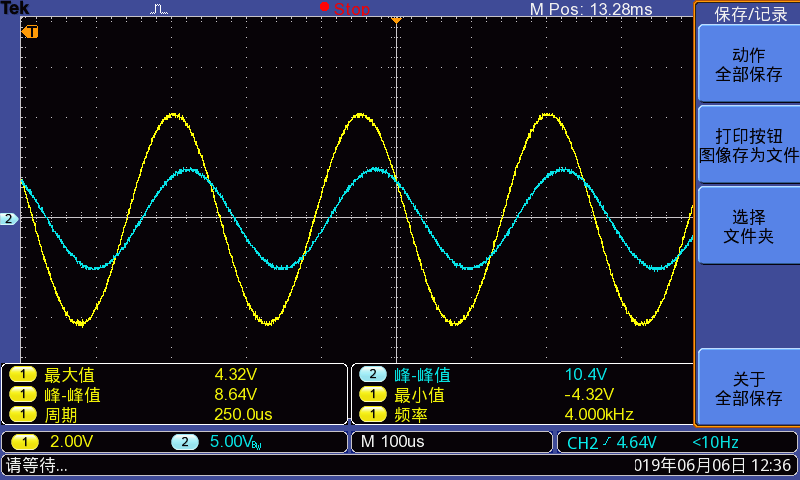
\includegraphics[width=\linewidth]{TEK28.png}
		\caption{RC高通滤波器测量数据\arabic{subfigure}}
		\label{fig:RC高通滤波器测量数据\arabic{subfigure}}
	\end{subfigure}
\end{figure}
\addtocounter{figure}{-1}
\begin{figure}[htpb]
	\setcounter{sub}{\value{subfigure}}
	\begin{subfigure}[htpb]{.45\linewidth}
		\setcounter{subfigure}{\value{sub}}
		\centering
		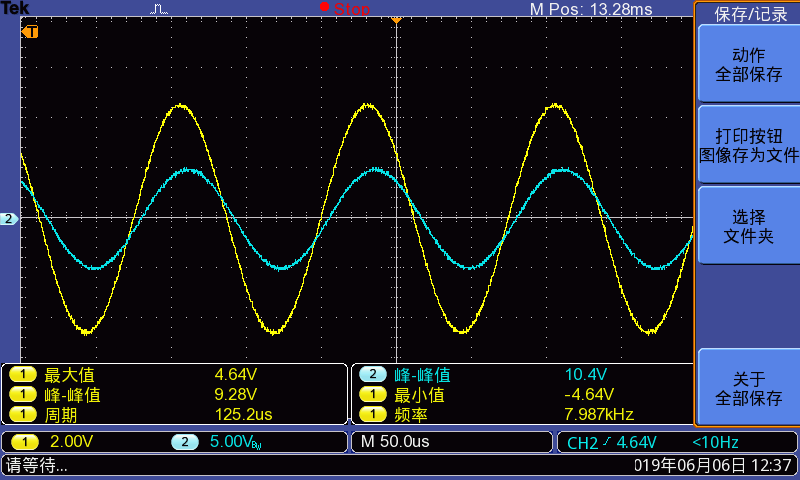
\includegraphics[width=\linewidth]{TEK29.png}
		\caption{RC高通滤波器测量数据\arabic{subfigure}}
		\label{fig:RC高通滤波器测量数据\arabic{subfigure}}
	\end{subfigure}
	\quad
	\begin{subfigure}[htpb]{.45\linewidth}
		\centering
		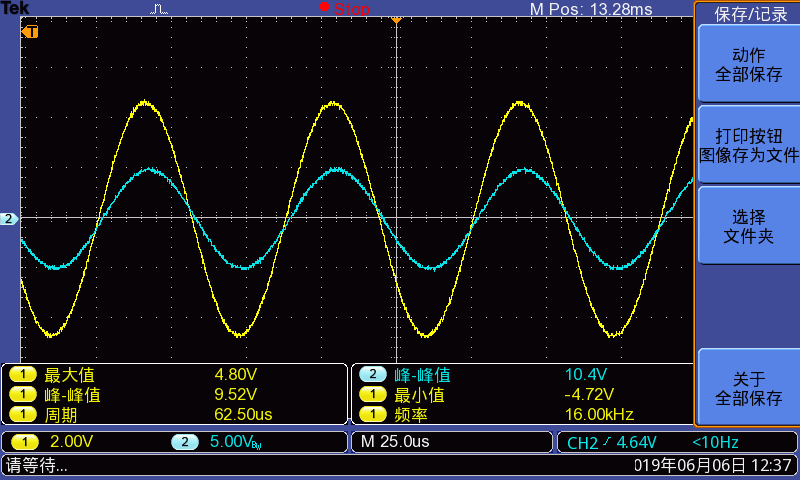
\includegraphics[width=\linewidth]{TEK2a.png}
		\caption{RC高通滤波器测量数据\arabic{subfigure}}
		\label{fig:RC高通滤波器测量数据\arabic{subfigure}}
	\end{subfigure}
	\caption{RC高通滤波器测量数据}
	\label{fig:RC高通滤波器测量数据}
\end{figure}
\begin{table}[htpb]
	\centering
	\caption{RC高通滤波器测量数据}
	\label{tab:RC高通滤波器测量数据}
	\csvreader[
	head to column names,
	tabular=|c|c|c|c|c|c|c|c|c|c|c|,
	table head=\hline,
	late after line=\\
	\hline
	]{src/2-5-1.csv}{}{ \a&\b&\c&\d&\e&\f&\g&\h&\i&\j&\k }
\end{table}
\subsection{RC低通滤波器的频响特性的测量}%
\label{sub:RC低通滤波器的频响特性的测量}
将信号源的输出(A)接实验板的IN2,滤波后的输出信号OUT2接示波器的输入(B)。根据被测电路的参数及系统的幅频特性,将输入信号的频率从低到高逐次改变十次以上(幅度保持$V_\text{ipp}=\SI{10}{V}$),逐个测量输出信号的峰峰值大小($V_\text{opp}$)及$\varphi(^{\circ})$,并将测量数据填入表\ref{tab:RC低通滤波器测量数据}:
\begin{table}[htpb]
	\centering
	\caption{RC低通滤波器测量数据}
	\label{tab:RC低通滤波器测量数据}
	\csvreader[
	head to column names,
	tabular=|c|c|c|c|c|c|c|c|c|c|c|,
	table head=\hline,
	late after line=\\
	\hline
	]{src/2-5-2.csv}{}{ \a&\b&\c&\d&\e&\f&\g&\h&\i&\j&\k }
\end{table}
\subsection{双TRC带阻滤波器的频响特性的测量}%
\label{sub:双TRC带阻滤波器的频响特性的测量}
将实验板上的两输入端IN1与IN2短接,输出端OUT1与OUT2短接;并将信号源的输出(A)接实验板输入(IN1)或(IN2),滤波后的输出OUT1或OUT2接示波器的输入(B)。根据被测电路的参数及系统的幅频特性,将输入信号的频率从低到高逐次改变二十次以上(幅度保持$ V_\text{ipp}=\SI{10}{V} $),逐个测量输出信号的峰峰值大小($ V_\text{opp} $)及$ \varphi(^{\circ}) $,并将测量数据填入表\ref{tab:双TRC带阻滤波器测量数据}:
\begin{table}[htpb]
	\centering
	\caption{双TRC带阻滤波器测量数据}
	\label{tab:双TRC带阻滤波器测量数据}
	\csvreader[
	head to column names,
	tabular=|c|c|c|c|c|c|c|c|c|c|c|,
	table head=\hline,
	late after line=\\
	\hline
	]{src/2-5-3.csv}{}{ \a&\b&\c&\d&\e&\f&\g&\h&\i&\j&\k }
\end{table}
\section{实验仪器及设备}%
\label{sec:实验仪器及设备\arabic{chapter}}
函数发生器一台 ,双踪示波器一台,实验板一块。
\section{实验报告要求}%
\label{sec:实验报告要求\arabic{chapter}}
\begin{Exercise}
	叙述实验内容及实验步骤。
\end{Exercise}
\begin{Answer}
	实验内容及实验步骤见第\ref{sec:实验内容及步骤\arabic{chapter}}节。
\end{Answer}
\begin{Exercise}
	整理实验数据,并以$ \lg f $为横坐标,$ V_{o}/V_{i} $为纵坐标,绘制三种滤波器的幅频特性曲线;以$ \lg f $为横坐标,$ \varphi(\Omega) $为纵坐标,绘制三种滤波器的相频特性曲线 。
\end{Exercise}
\begin{Answer}
	频响特性曲线见图\ref{fig:高通滤波实验波特图}。
\end{Answer}
\langCVfile[Matlab][code:lgfPlot.m][Matlab]{lgfPlot.m}{src/lgfPlot.m}
\langCVfile[Matlab][code:code272.m][Matlab]{code272.m}{src/code272.m}
\begin{figure}[htpb]
	\centering
	\matlablightfile{MATLAB Command Window}{src/code272.txt}
	\caption{运行界面}
	\label{fig:运行界面code272.m}
\end{figure}
\begin{figure}[htpb]
	\centering
	\begin{subfigure}[htpb]{.45\linewidth}
		\centering
		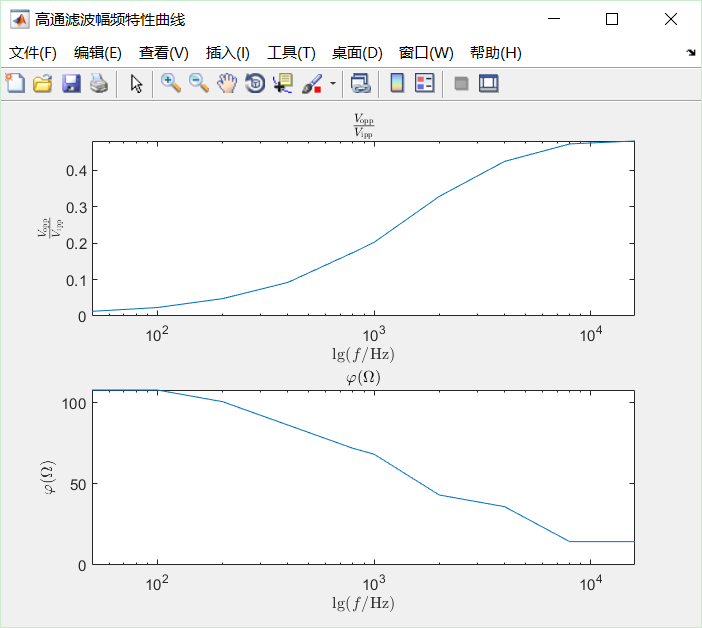
\includegraphics[width=\linewidth]{BodeHP.png}
		\caption{高通滤波实验波特图}
		\label{fig:高通滤波实验波特图}
	\end{subfigure}
	\quad
	\begin{subfigure}[htpb]{.45\linewidth}
		\centering
		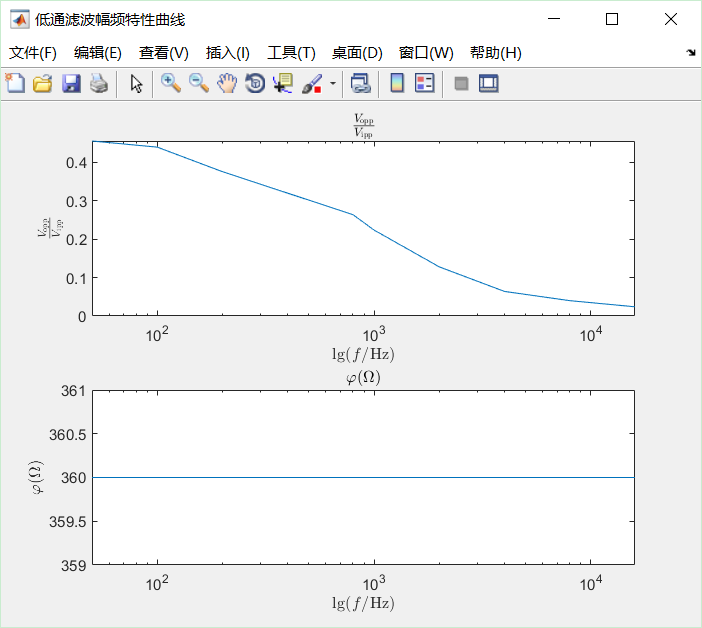
\includegraphics[width=\linewidth]{BodeLP.png}
		\caption{低通滤波实验波特图}
		\label{fig:低通滤波实验波特图}
	\end{subfigure}
	\begin{subfigure}[htpb]{.45\linewidth}
		\centering
		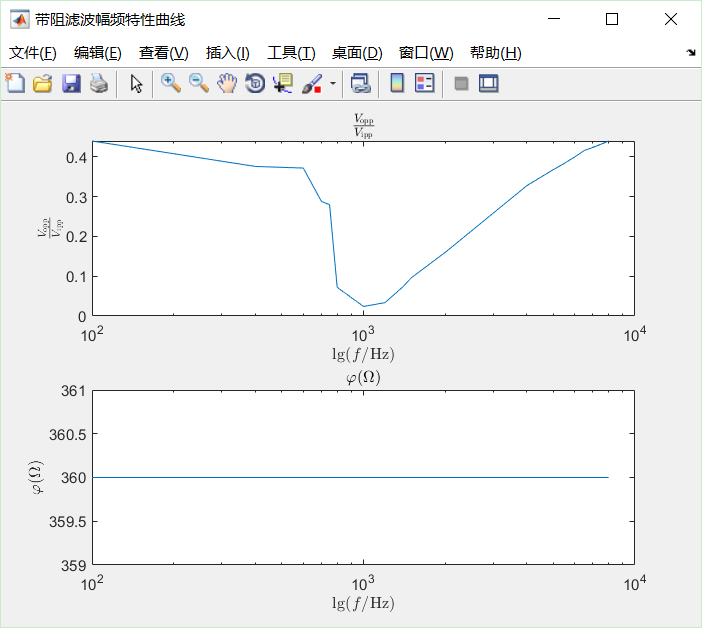
\includegraphics[width=\linewidth]{BodeBS.png}
		\caption{带阻滤波实验波特图}
		\label{fig:带阻滤波实验波特图}
	\end{subfigure}
	\caption{实验波特图}
	\label{fig:实验波特图}
\end{figure}
\begin{Exercise}
	将实验所得的频率响应特性曲线与仿真图进行比较;并将测得的各滤波器的截止频率与理论值进行比较,分析其结果是否一致,若误差较大则分析误差原因。
\end{Exercise}
\begin{Answer}
	仿真图见图\ref{fig:频响特性曲线}和\ref{fig:实验波特图},结果相对一致。
\end{Answer}


\chapter{信号通过线性系统}%
\label{cha:信号通过线性系统}

\section{实验目的}%
\label{sec:实验目的\arabic{chapter}}

\begin{enumerate}
	\item 观察对称方波通过线性系统后波形的失真,了解线性系统频率特性对信号传输的影响;
	\item 测试线性系统的时域特性——阶跃响应。
\end{enumerate}

\section{实验原理及方法}%
\label{sec:实验原理及方法\arabic{chapter}}

本实验所采用的激励信号为对称方波,此信号具有极丰富的频率分量,当这样的信号通过线性系统时,若系统的频率响应特性不满足无失真传输的条件,那么方波中的某些频率分量必然被抑制,造成输出信号与输入信号的不同(失真);若系统的频率响应特性不同则被抑制的频率亦会不同,输出信号的形状也不相同。

\begin{enumerate}
	\item 对称方波通过微分电路(高通滤波器)

		微分电路如图\ref{fig:微分电路}所示,该电路的时间常数为$ T=RC $,若输入的方波的脉宽$ \tau $远大于电路的时间常数$ T $,则输出的波形为尖脉冲;若方波的脉宽$ \tau $远小于电路的时间常数$ T $,则输出的波形近似方波如图\ref{fig:微分电路}所示。

		\begin{figure}[htpb]
			\centering
			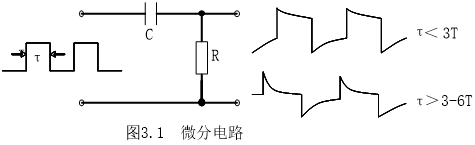
\includegraphics[width=0.8\linewidth]{3-2.png}
			\caption{微分电路}
			\label{fig:微分电路}
		\end{figure}

		从频域角度分析,微分电路实质上是一个高通滤波器,其系统函数为:$ H(s)= \dfrac{s}{s+ \dfrac{1}{RC} } $,其截止频率为:$ \Omega_\text{c}= \dfrac{1}{RC} $。

		当方波通过高通滤波器时,基波及低次谐波分量将受到衰减,从而产生平顶失真;而且$ RC $越小(截止频率越大)失真越大,即波形越尖;反之波形失真较小,波形较平坦。
	\item 对称方波通过积分电路(低通滤波器)

		积分电路如图\ref{fig:积分电路}所示,该电路的时间常数为$ T=RC $,若输入的方波的脉宽$ \tau $远大于电路的时间常数$ T $,则输出的波形近似方波;若方波的脉宽$ \tau $远小于电路的时间常数$ T $,则输出的精度大大降低,波形接近三角波如图\ref{fig:积分电路}所示。

		\begin{figure}[htpb]
			\centering
			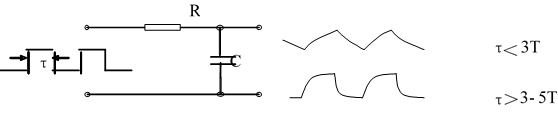
\includegraphics[width=0.8\linewidth]{3-2a.png}
			\caption{积分电路}
			\label{fig:积分电路}
		\end{figure}

		同样从频域角度分析,积分电路实质上是一个低通滤波器,其系统函数为:$ H(s)= \dfrac{1}{RC} \dfrac{1}{s+ \dfrac{1}{RC} } $,其截止频率为:$ \Omega_\text{c}= \dfrac{1}{RC} $。

		当方波通过低通滤波器时,高次谐波分量将受到衰减,因而输出信号中只有低频分量,因此输出波形的前沿变倾斜;而且$ RC $越大(截止频率越小),前沿倾斜越大,即波形失真越大;反之波形失真较小,波形较接近方波。
	\item 对称方波通过LC低通滤波器

		LC低通滤波器的电路如图\ref{fig:LC 低通滤波器}所示。

		\begin{figure}[htpb]
			\centering
			\includegraphics{LC.pdf}
			\caption{LC 低通滤波器}
			\label{fig:LC 低通滤波器}
		\end{figure}

		LC低通滤波器的截止频率为:$ \Omega_\text{c}=\dfrac{2}{\sqrt{(L_1+L_2)C}} $

		当对称矩形脉冲(方波)通过低通滤波器时,频率高于$ f_\text{c} $的谐波分量将被截止(或衰减)到达不了输出端,只有$ f<f_\text{c}  $的低频分量可以到达输出端,所以当不同频率的方波通过此滤波器时,能通过的频率分量将不同;方波的频率越高,通过的频率分量越少即失真越大。

		\begin{enumerate}
			\item 若方波的基波分量$ f_1<f_\text{c} $,而三次谐波分量$ f_3<f_\text{c} $;则能通过的只有$ f_1 $,即输出端为正弦信号;
			\item 若方波的三次谐波分量$ f_3<f_\text{c} $,而五次谐波分量$ f_5<f_\text{c} $,则能通过的只有$ f_1 $,$ f_3 $,即输出端信号为基次和三次谐波的合成波形;
			\item 若方波的频率$ f<<f_\text{c} $,则通过的谐波分量大大增加输出波形更接近方波但此时在波形的前沿将出现一峰值这就是吉伯斯现象。
		\end{enumerate}
	\item 阶跃响应的观测

		阶跃响应则是指单位阶跃信号作用下系统的零状态响应。我们用冲激响应和阶跃响应来描述系统的时域特性。由于普通示波器无法捕捉到$ t=0 $时刻的瞬间跳变,所以我们用方波作为激励信号;只要方波的重复周期$ T_1 $足够大 ($ T_1>> $阶跃响应建立的时间$ t_r $) ,则方波前半周的信号就可以看成是阶跃信号,若将此方波通过系统其响应的前半周就可以认为是阶跃响应。本实验的线性系统为一串联谐振系统,如图\ref{fig:串联谐振电路}所示。

		\begin{figure}[htpb]
			\centering
			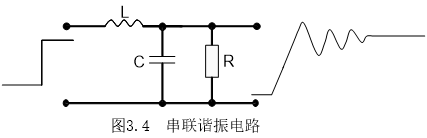
\includegraphics[width=0.8\linewidth]{3-2c.png}
			\caption{串联谐振电路}
			\label{fig:串联谐振电路}
		\end{figure}

		当方波加至串联谐振电路时,将引起电路的谐振,振荡的频率为$ \Omega_0=\dfrac{1}{\sqrt{LC}} $,此时只要满足方波的频率$ \Omega_1<<\Omega_0 $,就可以把响应的前半周认为是阶跃响应。
\end{enumerate}

\section{实验前预习内容}%
\label{sec:实验前预习内容\arabic{chapter}}

\begin{Exercise}
	计算微分电路的截止频率($ R=\SI{10}{k\ohm},C=\SI{1000}{pF} $),并画出幅频特性曲线。
\end{Exercise}

\begin{Answer}
	截止频率见图\ref{fig:运行界面code33.m},幅频特性曲线见图\subref{fig:微分电路幅频特性曲线}。
\end{Answer}

\begin{Exercise}
	计算积分电路的截止频率($ R=\SI{20}{k\ohm},C=\SI{1000}{pF} $),并画出幅频特性曲线。
\end{Exercise}

\begin{Answer}
	截止频率见图\ref{fig:运行界面code33.m},幅频特性曲线见图\subref{fig:积分电路幅频特性曲线}。
\end{Answer}

\begin{Exercise}
	计算LC低通滤波器的截止频率($ L=\SI{10}{mH},C=\SI{0.1}{\micro F} $)。
\end{Exercise}

\begin{Answer}
	截止频率见图\ref{fig:运行界面code33.m}。
\end{Answer}

\langCVfile[Matlab][code:code33.m][Matlab]{code33.m}{src/code33.m}

\begin{figure}[htpb]
	\centering
	\matlablightfile{MATLAB Command Window}{src/code33.txt}
	\caption{运行界面}
	\label{fig:运行界面code33.m}
\end{figure}

\begin{figure}[htpb]
	\centering
	\begin{subfigure}[htpb]{.45\linewidth}
		\centering
		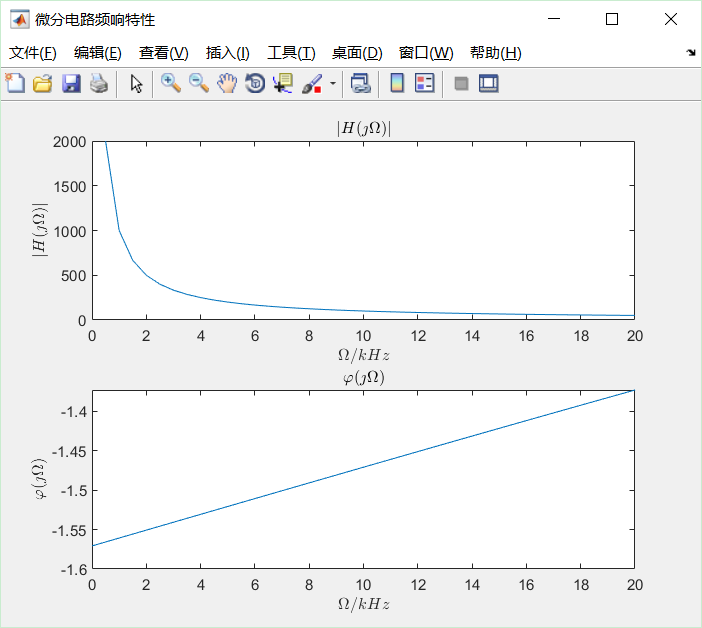
\includegraphics[width=\linewidth]{D.png}
		\caption{微分电路幅频特性曲线}
		\label{fig:微分电路幅频特性曲线}
	\end{subfigure}
	\quad
	\begin{subfigure}[htpb]{.45\linewidth}
		\centering
		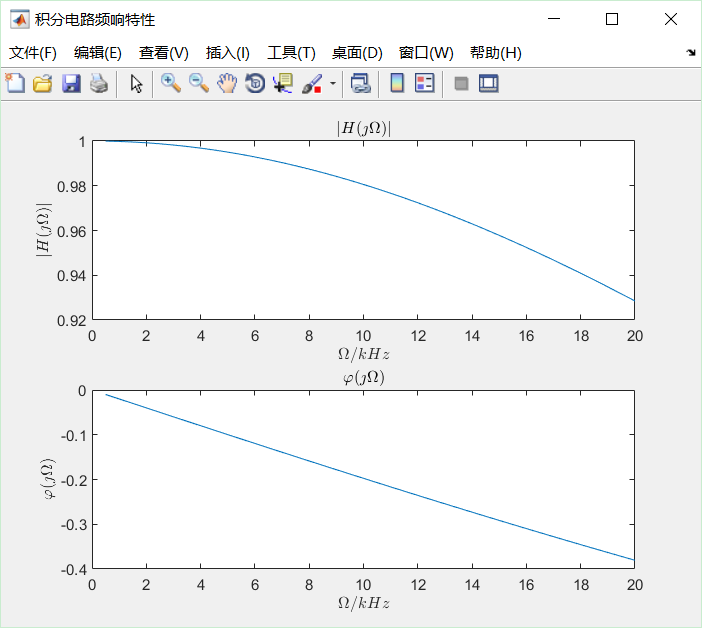
\includegraphics[width=\linewidth]{S.png}
		\caption{积分电路幅频特性曲线}
		\label{fig:积分电路幅频特性曲线}
	\end{subfigure}
	\caption{电路幅频特性曲线}
	\label{fig:电路幅频特性曲线}
\end{figure}

\begin{Exercise}
	用Matlab画出图\ref{fig:串联谐振电路}所示串联谐振电路的阶跃响应图形。
\end{Exercise}

\begin{Answer}
	阶跃响应波形见图\ref{fig:阶跃响应}。
\end{Answer}

\langCVfile[Matlab][code:code334.m][Matlab]{code334.m}{src/code334.m}

\begin{figure}[htpb]
	\centering
	\matlablightfile{MATLAB Command Window}{src/code334.txt}
	\caption{运行界面}
	\label{fig:运行界面code334.m}
\end{figure}

\begin{figure}[htpb]
	\centering
	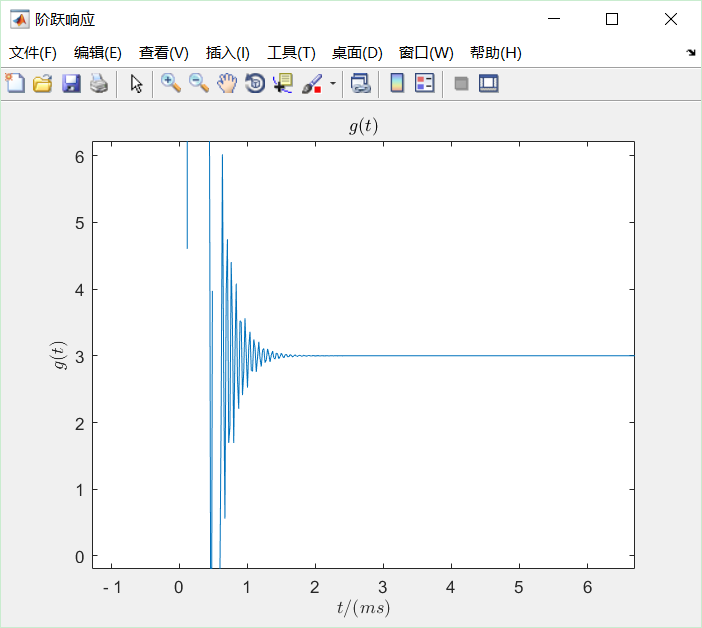
\includegraphics[width=0.6\linewidth]{stepResponse.png}
	\caption{阶跃响应}
	\label{fig:阶跃响应}
\end{figure}

\newpage

\section{实验原理图}%
\label{sec:实验原理图\arabic{chapter}}

\begin{figure}[htpb]
	\centering
	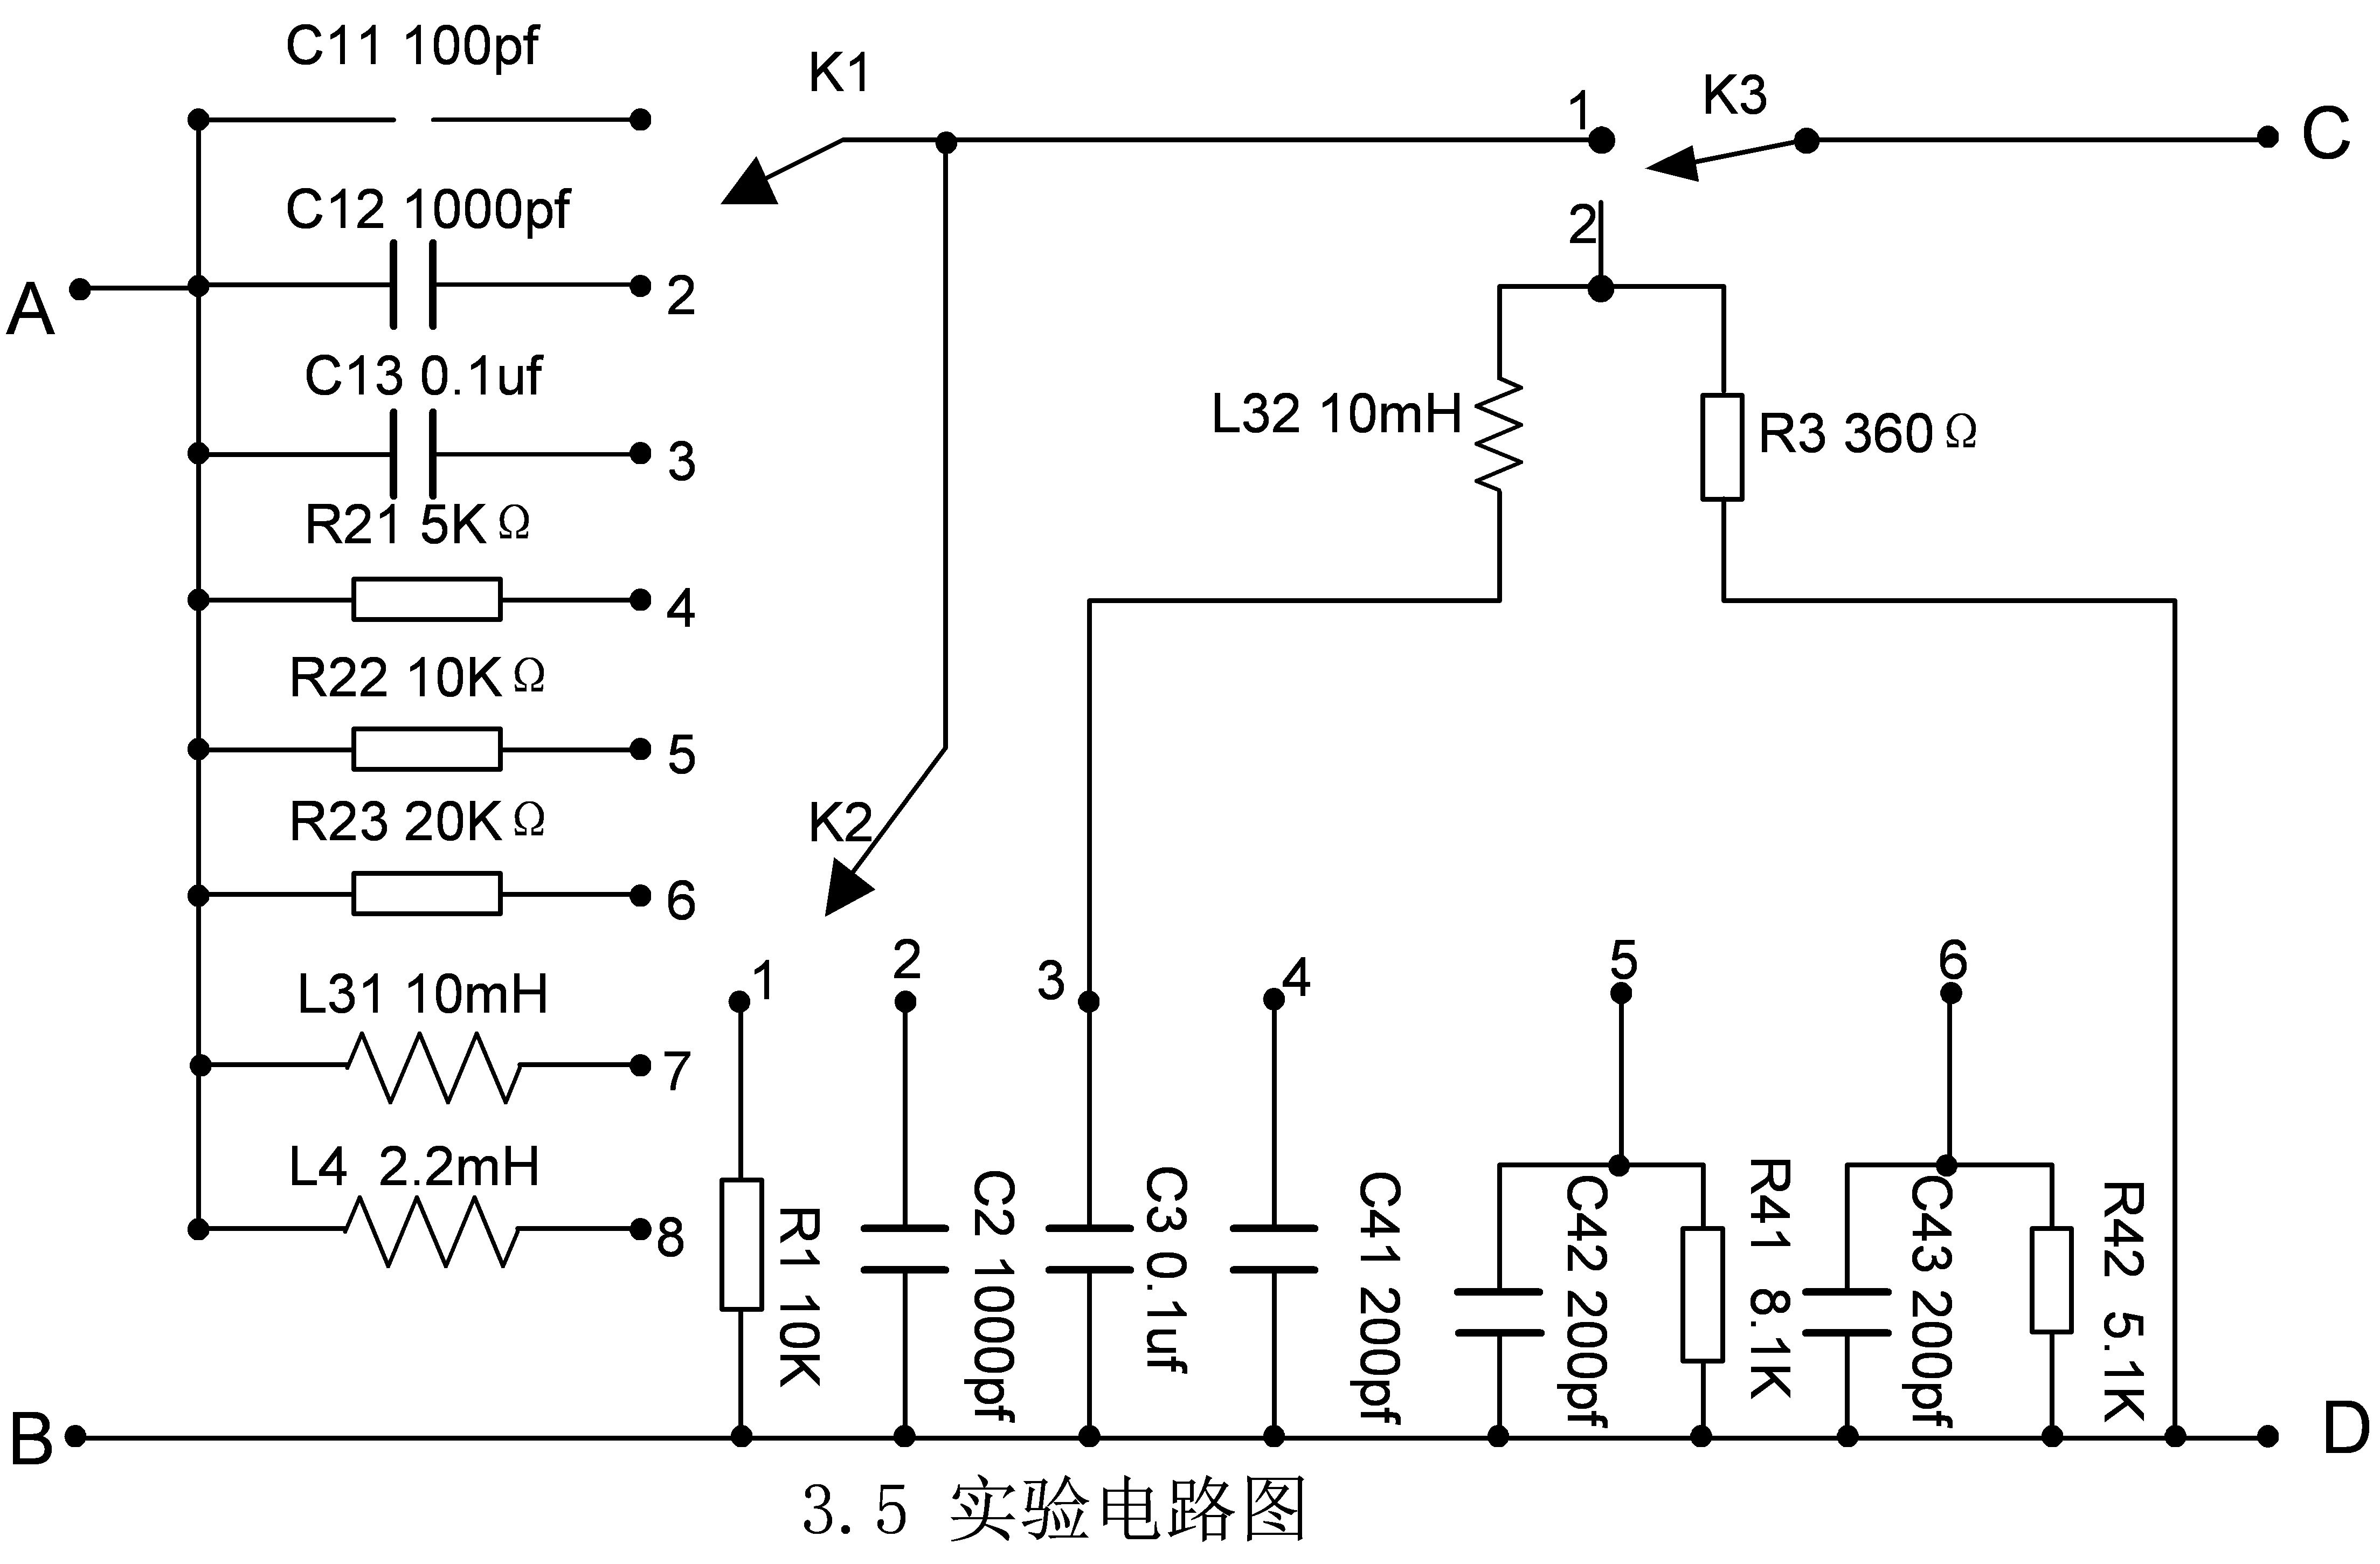
\includegraphics[width=0.6\linewidth]{3-4.png}
	\caption{实验原理图\arabic{chapter}}
	\label{fig:实验原理图\arabic{chapter}}
\end{figure}

\section{实验内容及步骤}%
\label{sec:实验内容及步骤\arabic{chapter}}

将函数发生器的输出CH1输出波形调为方波,频率调为\SI{10}{kHz},幅度调为$ V_\text{pp}=\SI{5}{V} $,并将此方波接实验板的A、B两点,示波器接实验板上的输出端CD两点。

\subsection{将电路接成微分电路,观察并记录波形}%
\label{sub:将电路接成微分电路,观察并记录波形}

将实验电路中的K2置于1,K3置于1, K1分别置于1,2,3,观察并记录波形;计算时间常数$ T=RC $的值,并与方波的脉宽$ \tau $进行比较说明时间常数T的变化对输出波形的影响。并从频域的角度(系统的频率特性)分析输出波形产生平顶失真的原因。

\begin{figure}[htpb]
	\centering
	\begin{subfigure}[htpb]{.31\linewidth}
		\centering
		\includegraphics[width=\linewidth]{TEK311.png}
		\caption{微分电路波形图\arabic{subfigure}}
		\label{fig:微分电路波形图\arabic{subfigure}}
	\end{subfigure}
	\quad
	\begin{subfigure}[htpb]{.31\linewidth}
		\centering
		\includegraphics[width=\linewidth]{TEK312.png}
		\caption{微分电路波形图\arabic{subfigure}}
		\label{fig:微分电路波形图\arabic{subfigure}}
	\end{subfigure}
	\quad
	\begin{subfigure}[htpb]{.31\linewidth}
		\centering
		\includegraphics[width=\linewidth]{TEK313.png}
		\caption{微分电路波形图\arabic{subfigure}}
		\label{fig:微分电路波形图\arabic{subfigure}}
	\end{subfigure}
	\caption{微分电路波形图}
	\label{fig:微分电路波形图}
\end{figure}

\subsection{将电路接成积分电路,观察并记录波形}%
\label{sub:将电路接成积分电路,观察并记录波形}

将实验电路中的K2置于2,K3置于1, K1分别置于4,5,6,观察并记录波形;计算时间常数$ T=RC $的值,并与方波的脉宽$ \tau $进行比较,说明时间常数T的变化对输出波形的影响。并从频域的角度(系统的频率特性)分析输出波形产生平顶失真的原因。

\begin{figure}[htpb]
	\centering
	\begin{subfigure}[htpb]{.31\linewidth}
		\centering
		\includegraphics[width=\linewidth]{TEK321.png}
		\caption{积分电路波形图\arabic{subfigure}}
		\label{fig:积分电路波形图\arabic{subfigure}}
	\end{subfigure}
	\quad
	\begin{subfigure}[htpb]{.31\linewidth}
		\centering
		\includegraphics[width=\linewidth]{TEK322.png}
		\caption{积分电路波形图\arabic{subfigure}}
		\label{fig:积分电路波形图\arabic{subfigure}}
	\end{subfigure}
	\quad
	\begin{subfigure}[htpb]{.31\linewidth}
		\centering
		\includegraphics[width=\linewidth]{TEK323.png}
		\caption{积分电路波形图\arabic{subfigure}}
		\label{fig:积分电路波形图\arabic{subfigure}}
	\end{subfigure}
	\caption{积分电路波形图}
	\label{fig:积分电路波形图}
\end{figure}

\subsection{将电路接成LC低通滤波器,观察并记录波形}%
\label{sub:将电路接成LC低通滤波器,观察并记录波形}

将实验电路中的K1置于7,K2置于3, K3置于2,观察并记录波形;然后改变信号源的频率 使之分别满足下面三个条件:\ding{172}$ f<f_\text{c}<3f $,\ding{173}$ 3f<f_\text{c}<5f $,\ding{174}$ f<<f_\text{c}(f_\text{c}=\SI{7.1}{kHz})$;分别记录三种情况下的输出波形,并从频域角度进行解释。

\begin{figure}[htpb]
	\centering
	\begin{subfigure}[htpb]{.31\linewidth}
		\centering
		\includegraphics[width=\linewidth]{TEK331.png}
		\caption{LC低通滤波器波形图\arabic{subfigure}}
		\label{fig:LC低通滤波器波形图\arabic{subfigure}}
	\end{subfigure}
	\quad
	\begin{subfigure}[htpb]{.31\linewidth}
		\centering
		\includegraphics[width=\linewidth]{TEK332.png}
		\caption{LC低通滤波器波形图\arabic{subfigure}}
		\label{fig:LC低通滤波器波形图\arabic{subfigure}}
	\end{subfigure}
	\quad
	\begin{subfigure}[htpb]{.31\linewidth}
		\centering
		\includegraphics[width=\linewidth]{TEK333.png}
		\caption{LC低通滤波器波形图\arabic{subfigure}}
		\label{fig:LC低通滤波器波形图\arabic{subfigure}}
	\end{subfigure}
	\caption{LC低通滤波器波形图}
	\label{fig:LC低通滤波器波形图}
\end{figure}

\subsection{将电路接成串联谐振回路,观察阶跃响应波形并记录}%
\label{sub:将电路接成串联谐振回路,观察阶跃响应波形并记录}

首先将信号源的频率调回\SI{10}{kHz},K1置于8,K3置于1,K2分别置于4,5,6,观察电路在不同损耗电阻值时的阶跃响应波形并记录。

\begin{figure}[htpb]
	\centering
	\begin{subfigure}[htpb]{.31\linewidth}
		\centering
		\includegraphics[width=\linewidth]{TEK341.png}
		\caption{串联谐振回路波形图\arabic{subfigure}}
		\label{fig:串联谐振回路波形图\arabic{subfigure}}
	\end{subfigure}
	\quad
	\begin{subfigure}[htpb]{.31\linewidth}
		\centering
		\includegraphics[width=\linewidth]{TEK342.png}
		\caption{串联谐振回路波形图\arabic{subfigure}}
		\label{fig:串联谐振回路波形图\arabic{subfigure}}
	\end{subfigure}
	\quad
	\begin{subfigure}[htpb]{.31\linewidth}
		\centering
		\includegraphics[width=\linewidth]{TEK343.png}
		\caption{串联谐振回路波形图\arabic{subfigure}}
		\label{fig:串联谐振回路波形图\arabic{subfigure}}
	\end{subfigure}
	\caption{串联谐振回路波形图}
	\label{fig:串联谐振回路波形图}
\end{figure}

\section{实验仪器及设备}%
\label{sec:实验仪器及设备\arabic{chapter}}

双踪示波器一台,函数发生器一台,实验板一块。

\section{实验报告要求}%
\label{sec:实验报告要求\arabic{chapter}}

\begin{Exercise}
	叙述实验内容及实验步骤。
\end{Exercise}

\begin{Answer}
	实验内容及实验步骤见第\ref{sec:实验内容及步骤\arabic{chapter}}节。
\end{Answer}

\begin{Exercise}
	详细画出实验内容\ref{sub:将电路接成微分电路,观察并记录波形}至\ref{sub:将电路接成LC低通滤波器,观察并记录波形}中要求记录得的波形,并对所得波形进行相应的理论解释。
\end{Exercise}

\begin{Answer}
	实验内容\ref{sub:将电路接成微分电路,观察并记录波形}至\ref{sub:将电路接成LC低通滤波器,观察并记录波形}中要求记录得的波形见图\ref{fig:微分电路幅频特性曲线}、\ref{fig:积分电路幅频特性曲线}和\ref{fig:LC低通滤波器波形图}。微分电路是高通滤波,保留了大部分高频分量,高频分量影响变化速率,所以跳变处出现 Gibbs 现象;但丧失了大部低频分量,低频分量携带大部分能量,所以阶跃响应比方波面积减小很多;所以最终出现尖顶失真。积分电路是低通滤波,保留了大部分低频分量,低频分量携带大部分能量,所以阶跃响应比方波面积减小不多,比高频响应更接近方波;但丧失了大部分高频分量,高频分量影响变化速率,所以跳变处没有出现 Gibbs 现象;所以最终出现削顶失真。
\end{Answer}

\begin{Exercise}
	在实验内容\ref{sub:将电路接成串联谐振回路,观察阶跃响应波形并记录}中,比较满足同一条件时信号频率取得较低和相对较高时的两种输出波形。
\end{Exercise}

\begin{Answer}
	信号频率较低时输出波形振荡较平缓。信号频率较高时输出波形振荡较剧烈。
\end{Answer}

\begin{Exercise}
	实验中的LC低通滤波器的过渡带宽如何确定。
\end{Exercise}

\begin{Answer}
	过渡带宽是处于通带和止带之间的数字频率宽度,即$ |w_p-w_s| $。在示波器上测量通带边界点和相邻的止带边界点的距离就是过渡带宽。
\end{Answer}

\begin{Exercise}
	画出实验内容\ref{sub:将电路接成串联谐振回路,观察阶跃响应波形并记录}中观察到的不同损耗时的波形,并说明电路中的电阻$ R $对输出波形有何影响。
\end{Exercise}

\begin{Answer}
	实验内容\ref{sub:将电路接成串联谐振回路,观察阶跃响应波形并记录}中观察到的不同损耗时的波形见图\ref{fig:串联谐振电路}。$ R $越大阶跃响应越接近方波。$ R $越小阶跃响应越接近正弦波。
\end{Answer}

\begin{Exercise}
	将实验内容\ref{sub:将电路接成串联谐振回路,观察阶跃响应波形并记录}中观察到输出波形的前半周与仿真的阶跃响应波形进行比较。
\end{Exercise}

\begin{Answer}
	实验内容\ref{sub:将电路接成串联谐振回路,观察阶跃响应波形并记录}中观察到输出波形见图\ref{fig:串联谐振回路波形图},仿真的阶跃响应波形见图\ref{fig:阶跃响应}。仿真时有意取了接近子图\subref{fig:串联谐振回路波形图2}的$ R, L, C $的值。
\end{Answer}


\chapter{信号的采样和采样定理}%
\label{cha:信号的采样和采样定理}

\section{实验目的}%
\label{sec:实验目的\arabic{chapter}}

\begin{enumerate}
	\item 掌握对连续时间信号进行采样的方法,了解采样信号的频谱的特点;
	\item 验证采样定理。
\end{enumerate}

\section{实验原理及方法}%
\label{sec:实验原理及方法\arabic{chapter}}

\begin{enumerate}
	\item 所谓采样信号是对连续时间信号每隔一定的时间抽取一次函数值而组成的一离散时间信号,采样信号$ f_\text{s} $可以表示成连续时间信号$ f(t) $与采样脉冲序列$ p(t) $的乘积,即:

		\begin{align}
			f_\text{s}(t)=f(t)p(t)
		\end{align}

		若采样脉冲序列$ p(t) $是以$ T_\text{s} $为周期的窄脉冲串,称为脉冲采样,$ T_\text{s} $的倒数$ f_\text{s} $为采样频率。$ f_\text{s},f(t),p(t) $的波形如图\ref{fig:矩形脉冲采样信号的频谱}所示:

		\begin{figure}[htpb]
			\centering
			\includegraphics[width=0.8\linewidth]{4-2.png}
			\caption{矩形脉冲采样信号的频谱}
			\label{fig:矩形脉冲采样信号的频谱}
		\end{figure}

		如连续信号的频谱为$ F(\jmath\Omega) $,则采样信号的频谱为$ F_\text{s}(\jmath\Omega) $其波形也见图\ref{fig:矩形脉冲采样信号的频谱}所示:其表达式为:

		\begin{align}
			F_\text{s}(\jmath\Omega)=\sum\limits_{n=-\infty}^{+\infty}P_nF\big(\jmath(\Omega-n\Omega_\text{s})\big)
		\end{align}

		上式表明,采样信号的频谱$ F_\text{s}(\jmath\Omega) $可以看成由采样信号的频谱$ F_\text{s}(\jmath\Omega) $以采样频率$ \Omega_\text{s} $为间隔周期延拓而得到的,在周期延拓过程中幅度被$ P_n $加权。当采样脉冲$ p(t) $是周期矩形脉冲时,采样信号的频谱为:

		\begin{align}
			F_\text{s}(\jmath\Omega)=\dfrac{E\tau}{T}\sum\limits_{n=-\infty}^{+\infty}\text{Sa}(\dfrac{n\Omega\tau}{2})F\big(\jmath(\Omega-n\Omega_\text{s})\big)
		\end{align}

	\item 采样信号在一定的条件下可以恢复出原信号。由采样定理可知,要恢复出原信号首先必须满足$ f_\text{s}>f_\text{m} $,其中$ f_\text{s} $为采样频率,$ f_\text{m} $为原信号的最高频率分量;在此前提下,用一截止频率为$ f_\text{c} $的低通滤波器滤除采样信号中的高频分量则可得到原信号。其中:

		\begin{align}
			f_\text{m}\leqslant f_\text{c}\leqslant f_\text{s}-f_\text{m}
		\end{align}

		当采样频率不满足采样定理,即$ f_\text{s}<2f_\text{m} $时,采样信号的频谱会发生混叠,原信号无法恢复。

		然而,仅包含有限频率的信号极少,而包含较多频率的信号即使在满足采样定理时,恢复后发生失真亦是难免的。
	\item 为了实现对连续信号的采样和采样信号的复原,可以采用图\ref{fig:信号的采样与恢复}的方案。

		\begin{figure}[htpb]
			\centering
			\includegraphics{sample.pdf}
			\caption{信号的采样与恢复}
			\label{fig:信号的采样与恢复}
		\end{figure}

		抗混叠滤波器用来防止原信号频谱过宽而造成采样后信号频谱的混叠,如果实验中采用的信号的频带较窄,则可不用此滤波器;采样器有多种实现电路,本实验中采用运算放大器组成模拟乘法器;重构滤波器为——低通滤波器,可用有源的也可用无源的,本实验中采用简单的$ \pi $型LC低通滤波器,如图\ref{fig:pi 型低通滤波器}所示:

		\begin{figure}[htpb]
			\centering
			\includegraphics{LC.pdf}
			\caption{$ \pi $型低通滤波器}
			\label{fig:pi 型低通滤波器}
		\end{figure}

		其截止频率$ f_\text{c}=\dfrac{1}{\pi\sqrt{LC}} $,标称特性阻抗$ R_\text{ld}=\sqrt{\dfrac{L}{C}} $,若给定$ R_\text{ld} $和$ f_\text{c} $就可按下式计算出元件的数值。

		\begin{align}
			L&=\dfrac{R_\text{ld}}{\pi f_\text{c}}\\
			C&=\dfrac{1}{\pi f_\text{c}R_\text{ld}}
		\end{align}

\end{enumerate}

\section{实验前预习内容}%
\label{sec:实验前预习内容\arabic{chapter}}

\begin{Exercise}
	若连续时间信号是频率为\SI{5}{kHz}的正弦波,采样脉冲$ p(t) $为$ T_\text{s}=\SI{40}{\micro s} $的窄脉冲,试求出采样信号$ f_\text{s}(t) $的频谱。
\end{Exercise}

\langCVfile[Matlab][code:code431.m][Matlab]{code431.m}{src/code431.m}

\begin{figure}[htpb]
	\centering
	%\matlablightfile{MATLAB Command Window}{src/code431.txt}
	\caption{运行界面}
	\label{fig:运行界面code431.m}
\end{figure}

\begin{Exercise}
	设计一$ \pi $型低通滤波器,截止频率为\SI{5}{kHz}, $ R_\text{ld} $为$ \SI{2}{k\ohm} $。
\end{Exercise}

\begin{Exercise}
	若连续时间信号是频率为\SI{1}{kHz}的三角波,估算其有效的频带宽度。该信号经重复频率为$ f_\text{s} $的周期脉冲采样后,若希望通过低通滤波器后的信号失真较小,则采样频率和低通滤波器的截止频率应分别取多少?试设计一满足上述要求的低通滤波器。
\end{Exercise}

\section{实验原理图}%
\label{sec:实验原理图\arabic{chapter}}

\begin{figure}[htpb]
	\centering
	\includegraphics[width=0.8\linewidth]{4-4.png}
	\caption{实验原理图\arabic{chapter}}
	\label{fig:实验原理图\arabic{chapter}}
\end{figure}

\section{实验内容及步骤}%
\label{sec:实验内容及步骤\arabic{chapter}}

\subsection{观察采样信号的波形}%
\label{sub:观察采样信号的波形}

\begin{enumerate}
	\item 将信号源的一路输出调为三角波,频率调为\SI{500}{Hz}作为被采样信号,另一路调为窄脉冲,频率调为\SI{1}{kHz}作为采样脉冲;
	\item 按原理图将两路信号分别加到实验板上的$ f(t) $及$ p(t) $端,用示波器同时观察$ f(t) $和$ f_\text{s}(t) $的波形;
	\item 将窄脉冲的频率(采样频率)改变为\SI{3}{kHz},\SI{6}{kHz}再次观察$ f(t) $和$ f_\text{s}(t) $的波形。
\end{enumerate}

\subsection{验证采样定理与信号恢复}%
\label{sub:验证采样定理与信号恢复}

首先将原理图中的开关K1,K2接1,然后进行下面的操作;

\begin{enumerate}
	\item\label{it:将信号源输出的三角波频率调为1kHz}将信号源输出的三角波频率调为\SI{1}{kHz},采样频率调为\SI{3}{kHz},并将采样信号 接低通滤波器的输入端($ \text{LPF}_\text{i} $), 示波器接低通滤波器的输出端($ \text{LPF}_\text{i} $)端,观察恢复后的波形;
	\item 将采样频率调为\SI{6}{kHz},其它条件不变,观察恢复后的波形;
	\item\label{it:将采样频率调为12kHz}将采样频率调为\SI{12}{kHz},其它条件不变,观察恢复后的波形;
\end{enumerate}

将原理图中的开关K1,K2接2,然后重复\ref{it:将信号源输出的三角波频率调为1kHz}至\ref{it:将采样频率调为12kHz}操作。

\section{实验仪器及设备}%
\label{sec:实验仪器及设备\arabic{chapter}}

双踪示波器一台,函数发生器一台,稳压电源一台,实验板一块。

\section{实验报告要求}%
\label{sec:实验报告要求\arabic{chapter}}

\begin{Exercise}
	绘出实验内容\ref{sub:观察采样信号的波形}中的$ f(t) $和$ f_\text{s}(t) $的波形。
\end{Exercise}

\begin{Exercise}
	绘出实验内容\ref{sub:观察采样信号的波形}中三种不同采样频率下的$ f(t) $和$ f_\text{s}(t) $的波形;比较后得出结论。
\end{Exercise}

\begin{Exercise}
	用Matlab画出对频率为\SI{1}{kHz}的正弦波和频率为\SI{3}{kHz}三角波用采样频率为\SI{6}{kHz}进行理想采样后的时域图和频谱图。
\end{Exercise}

\langCVfile[Matlab][code:code473.m][Matlab]{code473.m}{src/code473.m}

\begin{figure}[htpb]
	\centering
	\matlablightfile{MATLAB Command Window}{src/code473.txt}
	\caption{运行界面}
	\label{fig:运行界面code473.m}
\end{figure}

\begin{figure}[htpb]
	\centering
	\begin{subfigure}[htpb]{.45\linewidth}
		\centering
		%\includegraphics[width=\linewidth]{sine.png}
		\caption{正弦波时域图和频域图}
		\label{fig:正弦波时域图和频域图}
	\end{subfigure}
	\quad
	\begin{subfigure}[htpb]{.45\linewidth}
		\centering
		%\includegraphics[width=\linewidth]{triangle.png}
		\caption{三角波时域图和频域图}
		\label{fig:三角波时域图和频域图}
	\end{subfigure}
	\quad
	\caption{时域图和频域图}
	\label{fig:时域图和频域图}
\end{figure}


\end{document}

